% Compile with XeLaTeX or LuaLaTeX
\documentclass[12pt,a4paper]{article}

\usepackage[a4paper,margin=2.5cm]{geometry}
\usepackage{fontspec}
\usepackage{polyglossia}
\setmainlanguage{greek}
\setotherlanguage{english}
\setmainfont{DejaVu Serif}
\setsansfont{DejaVu Sans}
\setmonofont{DejaVu Sans Mono}
\newfontfamily\greekfont[Script=Greek]{DejaVu Serif}
\newfontfamily\greekfontsf[Script=Greek]{DejaVu Sans}
\newfontfamily\greekfonttt[Script=Greek]{DejaVu Sans Mono}
\usepackage{graphicx}
\usepackage{array}
\usepackage{booktabs}
\usepackage{tabularx}
\usepackage{float}
\usepackage{amsmath}
\usepackage{hyperref}
\usepackage{caption}
\usepackage{pdflscape}
\usepackage{fancyhdr}

\hypersetup{
  colorlinks=true,
  linkcolor=black,
  urlcolor=blue
}

\pagestyle{fancy}
\fancyhf{}
\fancyfoot[C]{\thepage}
\renewcommand{\headrulewidth}{0pt}
\renewcommand{\footrulewidth}{0pt}
\fancypagestyle{plain}{
  \fancyhf{}
  \fancyfoot[C]{\thepage}
  \renewcommand{\headrulewidth}{0pt}
  \renewcommand{\footrulewidth}{0pt}
}

\setlength{\parindent}{0pt}
\setlength{\parskip}{0.65em}
\renewcommand{\arraystretch}{1.2}

\newcolumntype{L}{>{\raggedright\arraybackslash}X}
\newcolumntype{C}[1]{>{\centering\arraybackslash}p{#1}}

\begin{document}

\begin{titlepage}
\centering

{\Large Αριστοτέλειο Πανεπιστήμιο Θεσσαλονίκης\par}
{\large Τμήμα Μηχανολόγων Μηχανικών\par}
\vspace{1.8cm}

{\LARGE\bfseries Υπολογισμός Ψυκτικού Φορτίου Κατοικίας\par}
\vspace{0.5cm}
{\Large Report για τα υποερωτήματα α, β και γ της εργασίας\par}
\vspace{0.8cm}
{\large Κτίριο Γ1 -- Κάτοψη Ισογείου\par}
\vspace{1.6cm}

\begin{tabular}{>{\bfseries}p{4.2cm}p{9.2cm}}
Μάθημα: & Κλιματισμός \\
Θέμα: & Τεκμηρίωση κτιρίου, υπολογισμός ψυκτικών φορτίων και βασικός σχεδιασμός συστήματος κλιματισμού \\
Ονοματεπώνυμο: & Ρακοβαλής Παύλος \\
Α.Ε.Μ.: & 6931 \\
Τοποθεσία έργου: & Θεσσαλονίκη \\
Κλιματική ζώνη: & Ζώνη Γ' κατά Κ.Εν.Α.Κ. \\
\end{tabular}

\vfill
{\large \today\par}
\thispagestyle{fancy}
\end{titlepage}

\tableofcontents
\newpage

\section{Εισαγωγή / Σκοπός}

Η παρούσα εργασία εντάσσεται στο πλαίσιο του μαθήματος του Κλιματισμού και έχει ως
γενικό αντικείμενο τον \textbf{σχεδιασμό συστήματος κλιματισμού κατοικίας}, με
βάση τα ψυκτικά φορτία που εμφανίζονται κατά τη θερινή περίοδο. Η μελέτη αναπτύσσει
με ενιαίο τρόπο και τα τρία υποερωτήματα της εκφώνησης: από την τεκμηρίωση του
κτιρίου αναφοράς και τον υπολογισμό των ψυκτικών φορτίων με τη μέθοδο
\textenglish{CLTD} της \textenglish{ASHRAE}, μέχρι τον ψυχρομετρικό σχεδιασμό του
συστήματος και τη συγκριτική αξιολόγηση δύο εναλλακτικών στρατηγικών αερισμού.

Η συνολική εργασία οργανώνεται σε επτά διαδοχικές ενότητες, οι οποίες καλύπτουν
και τα τρία υποερωτήματα της εκφώνησης:

\begin{itemize}
\item η εισαγωγή και ο σκοπός της εργασίας,
\item ο πίνακας βασικών συμβόλων,
\item η αναλυτική παρουσίαση του κτιρίου προς μελέτη (υποερώτημα α),
\item ο αναλυτικός υπολογισμός των ψυκτικών φορτίων με τη μέθοδο \textenglish{CLTD} της \textenglish{ASHRAE} (υποερώτημα β),
\item ο βασικός ψυχρομετρικός σχεδιασμός του συστήματος κλιματισμού για τη συνθήκη αιχμής (υποερώτημα γ),
\item τα συμπεράσματα της μελέτης,
\item και η σχετική βιβλιογραφία.
\end{itemize}

Συνεπώς, ο βασικός στόχος του κειμένου είναι να καλύψει με ακρίβεια και με ενιαία
τεχνική ορολογία ολόκληρη την αλυσίδα της μελέτης:

\begin{itemize}
\item την τεκμηρίωση της γεωμετρίας, του εξωτερικού περιβλήματος και των θερμοφυσικών
χαρακτηριστικών των δομικών στοιχείων του κτιρίου αναφοράς,
\item τον προσδιορισμό των αισθητών και λανθανόντων ψυκτικών φορτίων για χαρακτηριστικές
ώρες της 21ης Ιουλίου και τον εντοπισμό της ώρας αιχμής,
\item τη χάραξη της ψυχρομετρικής διεργασίας και τον υπολογισμό των βασικών παραμέτρων
του συστήματος κλιματισμού (παροχές, σημείο προσαγωγής, \textenglish{Apparatus Dew Point (ADP)}, συντελεστής παράκαμψης),
\item και τη συγκριτική αξιολόγηση δύο εναλλακτικών στρατηγικών αερισμού (χαμηλή και υψηλή παροχή νωπού αέρα).
\end{itemize}

\subsection{Αντικείμενο της εργασίας}

Αντικείμενο της εργασίας είναι το \textbf{Κτίριο Γ1}, δηλαδή η κάτοψη ισογείου
κατοικίας που εξετάζεται στη Θεσσαλονίκη (Κλιματική Ζώνη Γ' κατά Κ.Εν.Α.Κ.) και
αποτελεί τη θερμική ζώνη αναφοράς. Για το συγκεκριμένο κτίριο και για τις
ψυκτικές συνθήκες σχεδιασμού της εκφώνησης (21η Ιουλίου, ώρες 12:00, 16:00 και
20:00):

\begin{itemize}
\item \textbf{Υποερώτημα α} -- τεκμηριώνεται η γεωμετρία της κάτοψης, ο
προσανατολισμός, τα ανοίγματα, οι ακαθάριστες και καθαρές επιφάνειες των
εξωτερικών τοίχων, οι συντελεστές θερμοπερατότητας \(U\) των βασικών δομικών
στοιχείων και ο μέσος συντελεστής θερμοπερατότητας \(U_m\) του εξεταζόμενου
κελύφους.
\item \textbf{Υποερώτημα β} -- υπολογίζονται τα αισθητά και τα λανθάνοντα
ψυκτικά φορτία ανά κατηγορία (τοίχοι, οροφή, αγωγή και ηλιακά κέρδη
ανοιγμάτων, εσωτερικά φορτία, αερισμός), εντοπίζεται η ώρα αιχμής,
σχολιάζεται η επίδραση κάθε παράγοντα και προτείνονται στοχευμένες παρεμβάσεις
βελτίωσης (σκίαση, μόνωση οροφής, αναβάθμιση κουφωμάτων, περιορισμός
διεισδύσεων).
\item \textbf{Υποερώτημα γ} -- σχεδιάζεται \textenglish{single-zone all-air}
σύστημα κλιματισμού και προσδιορίζονται οι παροχές, το σημείο ανάμιξης, το
σημείο προσαγωγής, το \textenglish{Apparatus Dew Point} και ο συντελεστής
παράκαμψης για δύο εναλλακτικές στρατηγικές αερισμού -- χαμηλή και υψηλή
παροχή νωπού αέρα -- ώστε να αναδειχθεί η επίδραση του αερισμού στη
διαστασιολόγηση της συσκευής.
\end{itemize}

\subsection{Βασική μεθοδολογική παραδοχή}

Αν και η αρχιτεκτονική κάτοψη περιλαμβάνει περισσότερους του ενός χώρους
(καθιστικό, τραπεζαρία, κουζίνα, WC και χώλ), για τους θερμικούς υπολογισμούς το
ισόγειο θα αντιμετωπιστεί ως \textbf{μία ενιαία θερμική ζώνη}. Αυτό σημαίνει ότι τα
εσωτερικά χωρίσματα δεν θεωρούνται στοιχεία με ουσιώδη θερμική ροή μεταξύ χώρων με
διαφορετικές συνθήκες λειτουργίας, αλλά εσωτερικοί διαχωρισμοί του ίδιου
κλιματιζόμενου όγκου. Η ίδια παραδοχή υιοθετείται και στον ψυχρομετρικό σχεδιασμό
του συστήματος κλιματισμού στην Ενότητα~5, όπου το κτίριο αντιμετωπίζεται ως
ενιαίος κλιματιζόμενος όγκος που εξυπηρετείται από μία κεντρική κλιματιστική
μονάδα. Η παραδοχή αυτή δεν αναιρεί τη σημασία της αρχιτεκτονικής διαρρύθμισης, η
οποία εξακολουθεί να είναι απαραίτητη για τον εντοπισμό των ανοιγμάτων, των
εκτεθειμένων δομικών στοιχείων και της χρήσης κάθε τμήματος του κτιρίου.

\section{Πίνακας βασικών συμβόλων}

\subsection{Γενικά σύμβολα και θερμικά μεγέθη}

\begin{table}[H]
\centering
\small
\caption{Βασικά σύμβολα που χρησιμοποιούνται στις Ενότητες 1--4}
\begin{tabularx}{\textwidth}{C{2.2cm} L C{2.8cm}}
\toprule
\textbf{Σύμβολο} & \textbf{Περιγραφή} & \textbf{Μονάδα} \\
\midrule
\(A\) & Επιφάνεια δομικού στοιχείου ή ανοίγματος & \(\mathrm{m^2}\) \\
\(A_{\text{ακ.}}\) & Ακαθάριστη επιφάνεια τοίχου πριν από την αφαίρεση ανοιγμάτων & \(\mathrm{m^2}\) \\
\(A_{\text{καθ.}}\) & Καθαρή επιφάνεια τοίχου μετά την αφαίρεση ανοιγμάτων & \(\mathrm{m^2}\) \\
\(A_{\text{ανοιγμ.}}\) & Επιφάνεια ανοίγματος ή συνολική επιφάνεια ανοιγμάτων & \(\mathrm{m^2}\) \\
\(U\) & Συντελεστής θερμοπερατότητας συγκεκριμένου δομικού στοιχείου & \(\mathrm{W/(m^2K)}\) \\
\(U_m\) & Μέσος συντελεστής θερμοπερατότητας του εξεταζόμενου κελύφους & \(\mathrm{W/(m^2K)}\) \\
\(L\) & Μήκος δομικού στοιχείου ή πλευράς κάτοψης & \(\mathrm{m}\) \\
\(H\) & Ύψος ορόφου & \(\mathrm{m}\) \\
\(P\) & Περίμετρος κάτοψης & \(\mathrm{m}\) \\
\midrule
\(A_{\text{δαπ.}}\) & Εμβαδόν δαπέδου ισογείου & \(\mathrm{m^2}\) \\
\(A_{\text{οροφ.}}\) & Εμβαδόν οροφής σε επαφή με εξωτερικό αέρα & \(\mathrm{m^2}\) \\
\(A_{\text{τοίχων}}\) & Συνολικό εμβαδόν εξωτερικών τοίχων & \(\mathrm{m^2}\) \\
\midrule
\(q\) & Ψυκτικό φορτίο ή επιμέρους θερμική επιβάρυνση & \(\mathrm{W}\) \\
\(T_i\) & Εσωτερική θερμοκρασία σχεδιασμού του κλιματιζόμενου χώρου & \({}^\circ\mathrm{C}\) \\
\(T_o\) & Εξωτερική θερμοκρασία αέρα την εξεταζόμενη ώρα & \({}^\circ\mathrm{C}\) \\
\(T_{o,\max}\) & Μέγιστη εξωτερική θερμοκρασία της ημέρας αναφοράς & \({}^\circ\mathrm{C}\) \\
\(T_{o,\mathrm{mean}}\) & Μέση εξωτερική θερμοκρασία της ημέρας αναφοράς & \({}^\circ\mathrm{C}\) \\
\(DR\) & Ημερήσια θερμοκρασιακή διακύμανση (\textenglish{Daily Range}) & \({}^\circ\mathrm{C}\) \\
\(CLTD\) & \textenglish{Cooling Load Temperature Difference} για αδιαφανή στοιχεία ή υαλοπίνακες & \({}^\circ\mathrm{C}\) \\
\(LM\) & Διόρθωση γεωγραφικού πλάτους και μήνα της μεθόδου CLTD & \({}^\circ\mathrm{C}\) \\
\(K\) & Συντελεστής διόρθωσης λόγω χρώματος επιφάνειας & -- \\
\(f\) & Συντελεστής διόρθωσης οροφής λόγω ροής αέρα στην ψευδοροφή & -- \\
\(SC\) & Συντελεστής σκίασης υαλοπινάκων (\textenglish{Shading Coefficient}) & -- \\
\((SHGF)_{\max}\) & Μέγιστος παράγοντας ηλιακού θερμικού κέρδους υαλοπίνακα & \(\mathrm{W/m^2}\) \\
\(CLF\) & Παράγοντας ψυκτικού φορτίου (\textenglish{Cooling Load Factor}) & -- \\
\(HG\) & Στιγμιαίο θερμικό κέρδος (\textenglish{Heat Gain}) & \(\mathrm{W}\) \\
\(N\) & Αριθμός ατόμων στον χώρο & -- \\
\(f_u\) & Συντελεστής χρήσης φωτισμού & -- \\
\(f_s\) & Ειδικός συντελεστής φωτισμού ανάλογα με τον τύπο λαμπτήρων & -- \\
\(ACH\) & Αριθμός εναλλαγών αέρα ανά ώρα (\textenglish{Air Changes per Hour}) & \(\mathrm{h^{-1}}\) \\
\(\dot{m}\) & Παροχή μάζας αέρα & \(\mathrm{kg/s}\) \\
\(C_p\) & Ειδική θερμοχωρητικότητα υγρού αέρα & \(\mathrm{J/(kgK)}\) \\
\(W_i, W_o\) & Λόγος υγρασίας εσωτερικού και εξωτερικού αέρα αντίστοιχα & \(\mathrm{kg_w/kg_{da}}\) \\
\(h_g\) & Ειδική ενθαλπία υδρατμών που χρησιμοποιείται στον λανθάνοντα υπολογισμό αερισμού & \(\mathrm{J/kg_w}\) \\
\bottomrule
\end{tabularx}
\end{table}

\subsection{Συμβολισμοί δομικών στοιχείων του κτιρίου}

Για τη συστηματική παρουσίαση του κτιρίου και την ομοιόμορφη αναφορά σε όλα τα επόμενα
βήματα της εργασίας, χρησιμοποιείται ένας απλός και συνεπής συμβολισμός για τα
δομικά στοιχεία του εξωτερικού περιβλήματος.

\begin{table}[H]
\centering
\small
\caption{Συμβολισμοί αδιαφανών και διαφανών στοιχείων}
\begin{tabularx}{\textwidth}{C{2.6cm} L}
\toprule
\textbf{Συμβολισμός} & \textbf{Ερμηνεία} \\
\midrule
\(W_{L\mathrm{B}}\) & Εξωτερικός αδιαφανής τοίχος βόρειας όψης \\
\(W_{L\mathrm{N}}\) & Εξωτερικός αδιαφανής τοίχος νότιας όψης \\
\(W_{L\mathrm{A}}\) & Εξωτερικός αδιαφανής τοίχος ανατολικής όψης \\
\(W_{L\Delta}\) & Εξωτερικός αδιαφανής τοίχος δυτικής όψης \\
\(R\) & Οροφή σε επαφή με εξωτερικό αέρα \\
\(F\) & Δάπεδο σε επαφή με το έδαφος \\
\(W_{i\mathrm{B}1}\) & Πρώτο παράθυρο βόρειας όψης \\
\(W_{i\mathrm{B}2}\) & Δεύτερο παράθυρο βόρειας όψης \\
\(W_{i\mathrm{N}}\) & Παράθυρο νότιας όψης \\
\(W_{i\mathrm{A}}\) & Μπαλκονόπορτα ανατολικής όψης \\
\(W_{i\Delta}\) & Μπαλκονόπορτα δυτικής όψης \\
\bottomrule
\end{tabularx}
\end{table}

\subsection{Σύμβολα ψυχρομετρίας και συστήματος κλιματισμού}

Στην ενότητα του σχεδιασμού του συστήματος κλιματισμού χρησιμοποιούνται πρόσθετοι
συμβολισμοί που αφορούν την ψυχρομετρική διεργασία, τις παροχές αέρα και τα φορτία
του ψυκτικού στοιχείου. Οι συμβολισμοί αυτοί έχουν \textbf{τοπική ισχύ} στην
Ενότητα~5 και δεν συγχέονται με τους αντίστοιχους συμβολισμούς των δομικών
στοιχείων του κελύφους.

\begin{table}[H]
\centering
\small
\caption{Σύμβολα ψυχρομετρίας και συστήματος κλιματισμού}
\begin{tabularx}{\textwidth}{C{2.8cm} L C{2.6cm}}
\toprule
\textbf{Σύμβολο} & \textbf{Ερμηνεία} & \textbf{Μονάδα} \\
\midrule
\(O\) & Κατάσταση εξωτερικού αέρα (\textenglish{Outdoor air}) & -- \\
\(R\) & Κατάσταση αέρα χώρου / επιστροφής (\textenglish{Room or Return air}) & -- \\
\(M\) & Κατάσταση σημείου ανάμιξης νωπού και ανακυκλοφορούμενου αέρα & -- \\
\(S\) & Κατάσταση σημείου προσαγωγής μετά το ψυκτικό στοιχείο & -- \\
\(ADP\) & \textenglish{Apparatus Dew Point} του ψυκτικού στοιχείου & -- \\
\(BF\) & Συντελεστής παράκαμψης του ψυκτικού στοιχείου (\textenglish{Bypass Factor}) & -- \\
\(SHR\) & Λόγος αισθητής θερμότητας (\textenglish{Sensible Heat Ratio}) & -- \\
\(\dot V_{\text{νωπ.}}\) & Παροχή νωπού αέρα & \(\mathrm{m^3/h}\) ή \(\mathrm{L/s}\) \\
\(\dot V_{\text{ανακ.}}\) & Παροχή ανακυκλοφορούμενου αέρα & \(\mathrm{m^3/h}\) ή \(\mathrm{L/s}\) \\
\(\dot V_{\text{ολ.}}\) & Συνολική παροχή προσαγόμενου αέρα & \(\mathrm{m^3/h}\) ή \(\mathrm{L/s}\) \\
\(\dot m\) & Μαζική παροχή ξηρού αέρα & \(\mathrm{kg/s}\) \\
\(h\) & Ειδική ενθαλπία υγρού αέρα & \(\mathrm{kJ/kg_{da}}\) \\
\(Q_{\text{coil,sens}}\) & Αισθητό φορτίο ψυκτικού στοιχείου & \(\mathrm{W}\) \\
\(Q_{\text{coil,lat}}\) & Λανθάνον φορτίο ψυκτικού στοιχείου & \(\mathrm{W}\) \\
\(Q_{\text{coil,total}}\) & Συνολικό φορτίο ψυκτικού στοιχείου & \(\mathrm{W}\) \\
\bottomrule
\end{tabularx}
\end{table}

\section{Κτίριο προς μελέτη}

\subsection{Σύντομη περιγραφή του κτιρίου}

Το εξεταζόμενο κτίριο είναι το \textbf{Κτίριο Γ1}, δηλαδή ισόγεια κατοικία ορθογωνικής
κάτοψης με εξωτερικές διαστάσεις \(10.00\,\mathrm{m} \times 14.50\,\mathrm{m}\).
Το συνολικό εμβαδόν του ισογείου ισούται με:

\[
A_{\text{δαπ.}} = 10.00 \times 14.50 = 145.00\,\mathrm{m^2}
\]

Το ύψος του ορόφου θεωρείται:

\[
H = 3.00\,\mathrm{m}
\]

Το κτίριο βρίσκεται στη \textbf{Θεσσαλονίκη}, η οποία ανήκει στην \textbf{Κλιματική Ζώνη Γ'}
κατά Κ.Εν.Α.Κ. Η πληροφορία αυτή είναι καθοριστική, επειδή από αυτήν εξαρτάται η επιλογή
των συντελεστών θερμοπερατότητας των δομικών στοιχείων που χρησιμοποιούνται στη μελέτη.

\subsection{Σκαρίφημα κάτοψης}

Στο Σχήμα~\ref{fig:floorplan} παρατίθεται η κάτοψη του κτιρίου, από την οποία προέκυψαν
όλα τα γεωμετρικά δεδομένα της εργασίας.

\begin{figure}[H]
\centering
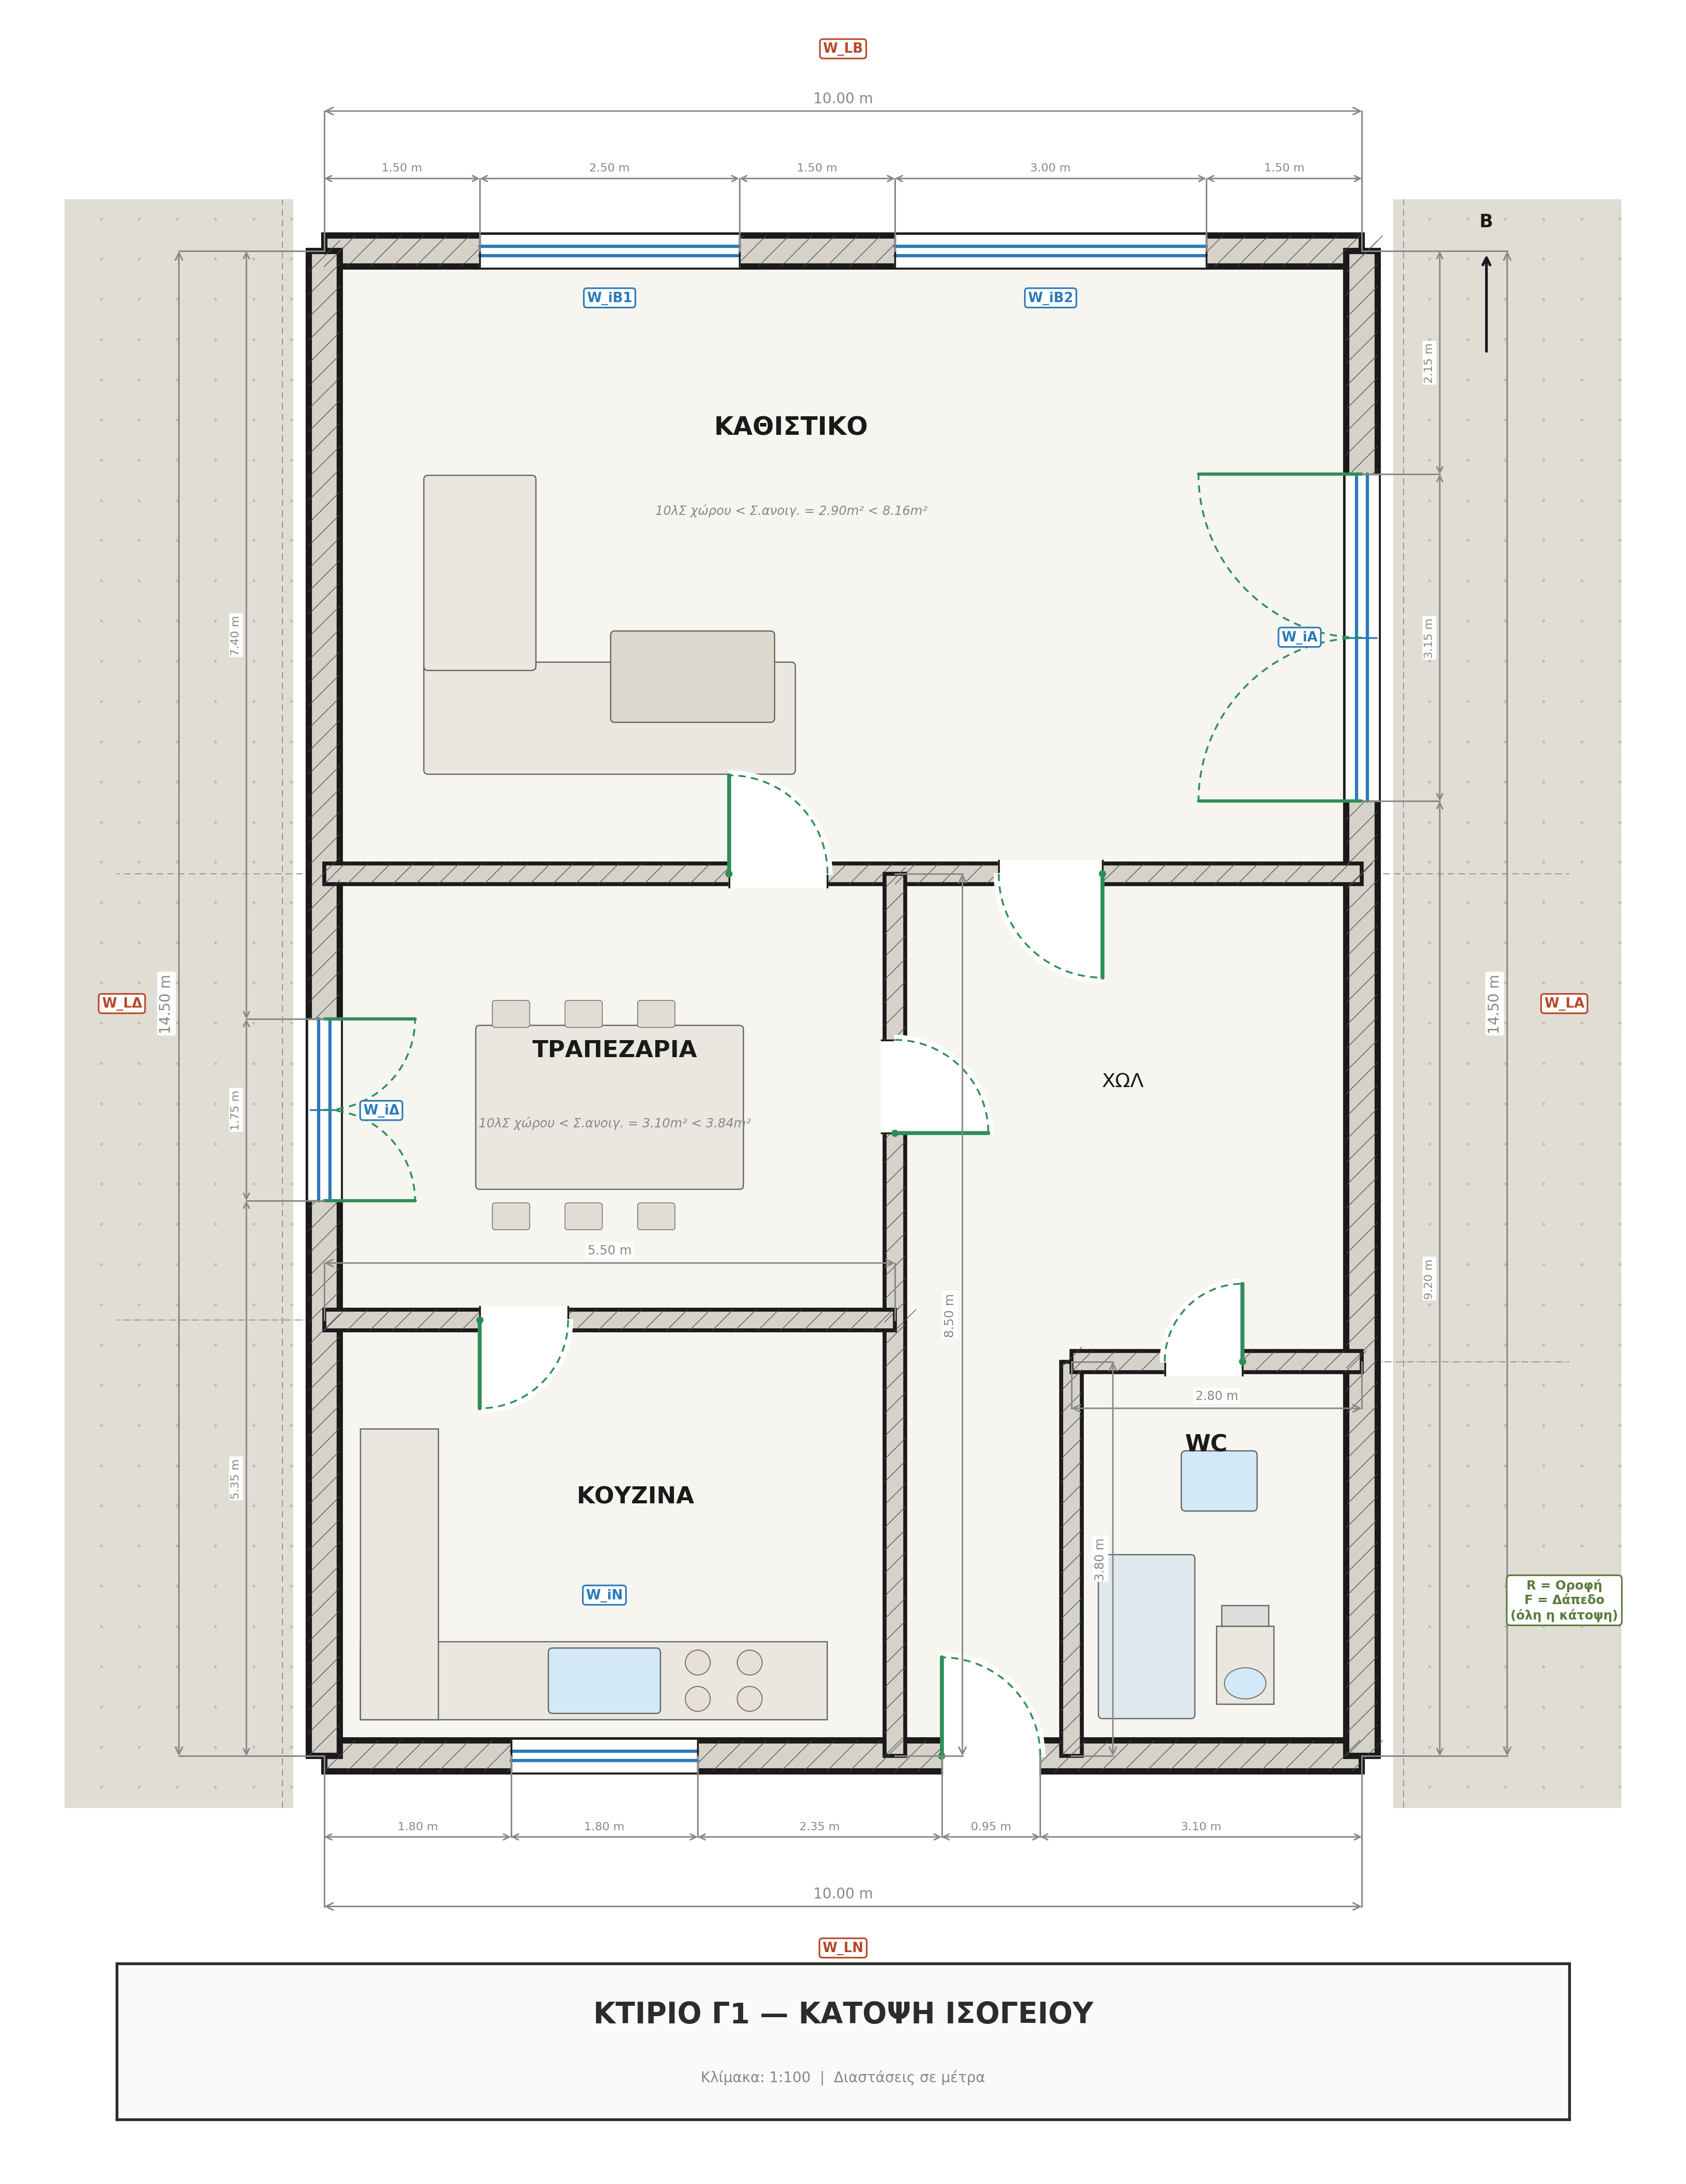
\includegraphics[width=0.84\textwidth]{floor_plan_G1.png}
\caption{Κάτοψη του Κτιρίου Γ1 που χρησιμοποιήθηκε ως βάση για την αποτύπωση του εξωτερικού περιβλήματος.}
\label{fig:floorplan}
\end{figure}

Η κάτοψη περιλαμβάνει πέντε βασικούς λειτουργικούς χώρους:

\begin{itemize}
\item καθιστικό,
\item τραπεζαρία,
\item κουζίνα,
\item WC,
\item χώλ.
\end{itemize}

\subsection{Γεωμετρικά χαρακτηριστικά της κάτοψης}

Οι βασικές γεωμετρικές πληροφορίες του κτιρίου συνοψίζονται στον επόμενο πίνακα.

\begin{table}[H]
\centering
\caption{Γενικά γεωμετρικά στοιχεία κτιρίου}
\begin{tabularx}{\textwidth}{L C{3.2cm}}
\toprule
\textbf{Μέγεθος} & \textbf{Τιμή} \\
\midrule
Συνολικές εξωτερικές διαστάσεις κάτοψης & \(10.00 \times 14.50\,\mathrm{m}\) \\
Συνολικό εμβαδόν δαπέδου / οροφής & \(145.00\,\mathrm{m^2}\) \\
Ύψος ορόφου & \(3.00\,\mathrm{m}\) \\
Πάχος εξωτερικών τοίχων & \(0.30\,\mathrm{m}\) \\
Πάχος εσωτερικών τοίχων & \(0.20\,\mathrm{m}\) \\
Περίμετρος κάτοψης & \(2 \times (10.00 + 14.50) = 49.00\,\mathrm{m}\) \\
\bottomrule
\end{tabularx}
\end{table}

\subsubsection{Επιμέρους εμβαδά λειτουργικών χώρων}

Με βάση τη γεωμετρία της κάτοψης, τα επιμέρους εμβαδά των χώρων υπολογίζονται ως εξής:

\begin{table}[H]
\centering
\small
\caption{Εμβαδά επιμέρους χώρων}
\begin{tabularx}{\textwidth}{L L C{2.8cm}}
\toprule
\textbf{Χώρος} & \textbf{Υπολογισμός} & \textbf{Εμβαδόν (\(\mathrm{m^2}\))} \\
\midrule
Καθιστικό & \(10.00 \times (14.50 - 8.50)\) & 60.00 \\
Τραπεζαρία & \(5.50 \times (8.50 - 4.20)\) & 23.65 \\
Κουζίνα & \(5.50 \times 4.20\) & 23.10 \\
WC & \((10.00 - 7.20) \times 3.80\) & 10.64 \\
Χώλ & \((10.00 - 5.50)\times(8.50 - 3.80) + (7.20 - 5.50)\times 3.80\) & 27.61 \\
\midrule
\textbf{Σύνολο} &  & \textbf{145.00} \\
\bottomrule
\end{tabularx}
\end{table}

Το άθροισμα των επιμέρους εμβαδών συμπίπτει με το συνολικό εμβαδόν της κάτοψης,
γεγονός που επιβεβαιώνει τη συνέπεια της γεωμετρικής αποτύπωσης.

\subsection{Προσανατολισμός του κτιρίου και ανοίγματα}

Για τις ανάγκες της μελέτης θεωρείται ότι:

\begin{itemize}
\item η άνω πλευρά της κάτοψης είναι η \textbf{βόρεια όψη},
\item η κάτω πλευρά είναι η \textbf{νότια όψη},
\item η δεξιά πλευρά είναι η \textbf{ανατολική όψη},
\item η αριστερή πλευρά είναι η \textbf{δυτική όψη}.
\end{itemize}

Από την κάτοψη προκύπτουν τα ακόλουθα διαφανή στοιχεία του εξωτερικού περιβλήματος:

\begin{table}[H]
\centering
\small
\caption{Ανοίγματα ανά όψη}
\begin{tabularx}{\textwidth}{L C{2.7cm} C{2.2cm} C{2.2cm} C{2.4cm}}
\toprule
\textbf{Άνοιγμα} & \textbf{Προσανατολισμός} & \textbf{Πλάτος (m)} & \textbf{Ύψος (m)} & \textbf{Εμβαδόν (\(\mathrm{m^2}\))} \\
\midrule
Παράθυρο Π1 -- Καθιστικό & Βορράς & 2.50 & 1.40 & 3.50 \\
Παράθυρο Π2 -- Καθιστικό & Βορράς & 3.00 & 1.40 & 4.20 \\
Παράθυρο Π3 -- Κουζίνα & Νότος & 1.80 & 1.40 & 2.52 \\
Μπαλκονόπορτα -- Καθιστικό & Ανατολή & 3.15 & 2.40 & 7.56 \\
Μπαλκονόπορτα -- Τραπεζαρία & Δύση & 1.75 & 2.40 & 4.20 \\
\midrule
\textbf{Σύνολο} &  &  &  & \textbf{21.98} \\
\bottomrule
\end{tabularx}
\end{table}

Οι απλές παραθυρικές επιφάνειες θεωρήθηκαν με ύψος \(1.40\,\mathrm{m}\), ενώ οι
μπαλκονόπορτες με ύψος \(2.40\,\mathrm{m}\). Η παραδοχή αυτή κρίθηκε αναγκαία, καθώς η
διαθέσιμη πληροφορία προέρχεται από κάτοψη και όχι από όψη του κτιρίου.

\subsection{Υποδήλωση ονομασίας δομικών στοιχείων}

Στο παρόν βήμα καταγράφονται αναλυτικά τα δομικά στοιχεία του εξωτερικού περιβλήματος
με τον αντίστοιχο συμβολισμό, τον προσανατολισμό τους, τη γεωμετρία τους και τις
επιφάνειές τους.

\subsubsection{Πίνακας Βήμα 1α -- Καταγραφή δομικών στοιχείων εξωτερικού περιβλήματος}

Για πληρότητα, παρατίθεται και ο συγκεντρωτικός πίνακας του Βήματος 1α, ο οποίος
αποτελεί την πλήρη απογραφή των αδιαφανών και διαφανών στοιχείων του κελύφους.

\begin{table}[H]
\centering
\scriptsize
\caption{Βήμα 1α -- Καταγραφή δομικών στοιχείων εξωτερικού περιβλήματος}
\resizebox{\textwidth}{!}{%
\begin{tabular}{p{1.9cm}p{2.8cm}p{4.2cm}p{2.3cm}p{2.2cm}p{1.5cm}p{1.8cm}p{1.7cm}p{2.0cm}}
\toprule
\textbf{Συμβολισμός} & \textbf{Τύπος στοιχείου} & \textbf{Υλικά κατασκευής} & \textbf{Προσανατολισμός} & \textbf{Μήκος/πλάτος (m)} & \textbf{Ύψος (m)} & \textbf{Επιφάνεια (\(\mathrm{m^2}\))} & \textbf{Αριθμός επιφανειών} & \textbf{Συντ. θερμοπερατότητας \(\mathrm{W/(m^2K)}\)} \\
\midrule
\multicolumn{9}{l}{\textbf{Αδιαφανή στοιχεία}} \\
\midrule
\(W_{L\mathrm{B}}\) & Εξωτερικός τοίχος & Τούβλο / μόνωση / σκυρόδεμα / επίχρισμα & Βορράς (Β) & 10.00 & 3.00 & 22.30 & 1 & 0.45 \\
\(W_{L\mathrm{N}}\) & Εξωτερικός τοίχος & Τούβλο / μόνωση / σκυρόδεμα / επίχρισμα & Νότος (Ν) & 10.00 & 3.00 & 27.48 & 1 & 0.45 \\
\(W_{L\mathrm{A}}\) & Εξωτερικός τοίχος & Τούβλο / μόνωση / σκυρόδεμα / επίχρισμα & Ανατολή (Α) & 14.50 & 3.00 & 35.94 & 1 & 0.45 \\
\(W_{L\Delta}\) & Εξωτερικός τοίχος & Τούβλο / μόνωση / σκυρόδεμα / επίχρισμα & Δύση (Δ) & 14.50 & 3.00 & 39.30 & 1 & 0.45 \\
\(R\) & Οροφή -- επαφή με εξωτερικό αέρα & Ο.Σ. / μόνωση / ασφαλτική επικάλυψη & -- & 10.00 \(\times\) 14.50 & -- & 145.00 & 1 & 0.40 \\
\(F\) & Δάπεδο -- επαφή με το έδαφος & Ο.Σ. / μόνωση / πλακάκι & -- & 10.00 \(\times\) 14.50 & -- & 145.00 & 1 & 0.60 \\
\midrule
\multicolumn{9}{l}{\textbf{Διαφανή στοιχεία}} \\
\midrule
\(W_{i\mathrm{B}1}\) & Παράθυρο -- καθιστικό & Αλουμίνιο / διπλό τζάμι & Βορράς (Β) & 2.50 & 1.40 & 3.50 & 1 & 2.40 \\
\(W_{i\mathrm{B}2}\) & Παράθυρο -- καθιστικό & Αλουμίνιο / διπλό τζάμι & Βορράς (Β) & 3.00 & 1.40 & 4.20 & 1 & 2.40 \\
\(W_{i\mathrm{N}}\) & Παράθυρο -- κουζίνα & Αλουμίνιο / διπλό τζάμι & Νότος (Ν) & 1.80 & 1.40 & 2.52 & 1 & 2.40 \\
\(W_{i\mathrm{A}}\) & Μπαλκονόπορτα (δίφυλλη) -- καθιστικό & Αλουμίνιο / διπλό τζάμι & Ανατολή (Α) & 3.15 & 2.40 & 7.56 & 1 & 2.40 \\
\(W_{i\Delta}\) & Μπαλκονόπορτα (δίφυλλη) -- τραπεζαρία & Αλουμίνιο / διπλό τζάμι & Δύση (Δ) & 1.75 & 2.40 & 4.20 & 1 & 2.40 \\
\midrule
\multicolumn{6}{r}{\textbf{Σύνολο αδιαφανών επιφανειών}} & \textbf{415.02} & \multicolumn{2}{l}{} \\
\multicolumn{6}{r}{\textbf{Σύνολο διαφανών επιφανειών}} & \textbf{21.98} & \multicolumn{2}{l}{} \\
\bottomrule
\end{tabular}%
}
\end{table}

\noindent Ο παραπάνω πίνακας είναι η πλήρης μορφή της καταγραφής του εξωτερικού
περιβλήματος. Για λόγους αναγνωσιμότητας, στη συνέχεια η ίδια πληροφορία αναλύεται
και σε επιμέρους πίνακες αδιαφανών και διαφανών στοιχείων.

\subsubsection{Αδιαφανή στοιχεία}

\begin{table}[H]
\centering
\small
\caption{Αδιαφανή δομικά στοιχεία του κτιρίου}
\begin{tabularx}{\textwidth}{C{2.6cm} L C{2.2cm} C{3.0cm} C{2.4cm}}
\toprule
\textbf{Συμβολισμός} & \textbf{Στοιχείο} & \textbf{Όψη} & \textbf{Διαστάσεις} & \textbf{Επιφάνεια (\(\mathrm{m^2}\))} \\
\midrule
\(W_{L\mathrm{B}}\) & Εξωτερικός τοίχος & Βορράς & \(10.00 \times 3.00\) & 22.30 \\
\(W_{L\mathrm{N}}\) & Εξωτερικός τοίχος & Νότος & \(10.00 \times 3.00\) & 27.48 \\
\(W_{L\mathrm{A}}\) & Εξωτερικός τοίχος & Ανατολή & \(14.50 \times 3.00\) & 35.94 \\
\(W_{L\Delta}\) & Εξωτερικός τοίχος & Δύση & \(14.50 \times 3.00\) & 39.30 \\
\(R\) & Οροφή σε επαφή με εξωτερικό αέρα & -- & \(10.00 \times 14.50\) & 145.00 \\
\(F\) & Δάπεδο σε επαφή με το έδαφος & -- & \(10.00 \times 14.50\) & 145.00 \\
\bottomrule
\end{tabularx}
\end{table}

\subsubsection{Διαφανή στοιχεία}

\begin{table}[H]
\centering
\small
\caption{Διαφανή δομικά στοιχεία του κτιρίου}
\begin{tabularx}{\textwidth}{C{2.6cm} L C{2.3cm} C{3.0cm} C{2.4cm}}
\toprule
\textbf{Συμβολισμός} & \textbf{Στοιχείο} & \textbf{Όψη} & \textbf{Διαστάσεις} & \textbf{Επιφάνεια (\(\mathrm{m^2}\))} \\
\midrule
\(W_{i\mathrm{B}1}\) & Παράθυρο καθιστικού & Βορράς & \(2.50 \times 1.40\) & 3.50 \\
\(W_{i\mathrm{B}2}\) & Παράθυρο καθιστικού & Βορράς & \(3.00 \times 1.40\) & 4.20 \\
\(W_{i\mathrm{N}}\) & Παράθυρο κουζίνας & Νότος & \(1.80 \times 1.40\) & 2.52 \\
\(W_{i\mathrm{A}}\) & Μπαλκονόπορτα καθιστικού & Ανατολή & \(3.15 \times 2.40\) & 7.56 \\
\(W_{i\Delta}\) & Μπαλκονόπορτα τραπεζαρίας & Δύση & \(1.75 \times 2.40\) & 4.20 \\
\bottomrule
\end{tabularx}
\end{table}

\subsection{Υπολογισμός επιφανειών εξωτερικού περιβλήματος}

\subsubsection{Ακαθάριστες επιφάνειες εξωτερικών τοίχων}

Οι ακαθάριστες επιφάνειες των τοίχων προκύπτουν από το μήκος κάθε όψης επί το ύψος:

\[
A_{\text{Β,ακ.}} = 10.00 \times 3.00 = 30.00\,\mathrm{m^2}
\]
\[
A_{\text{Ν,ακ.}} = 10.00 \times 3.00 = 30.00\,\mathrm{m^2}
\]
\[
A_{\text{Α,ακ.}} = 14.50 \times 3.00 = 43.50\,\mathrm{m^2}
\]
\[
A_{\Delta,\text{ακ.}} = 14.50 \times 3.00 = 43.50\,\mathrm{m^2}
\]

Άρα:

\[
A_{\text{τοίχων,ακ.}} = 30.00 + 30.00 + 43.50 + 43.50 = 147.00\,\mathrm{m^2}
\]

\subsubsection{Καθαρές επιφάνειες εξωτερικών τοίχων}

Οι καθαρές επιφάνειες προκύπτουν αφαιρώντας τα ανοίγματα από κάθε όψη:

\[
A_{\text{καθ.}} = A_{\text{ακ.}} - \sum A_{\text{ανοιγμ.}}
\]

Αναλυτικά:

\[
A_{\text{Β,καθ.}} = 30.00 - (3.50 + 4.20) = 22.30\,\mathrm{m^2}
\]
\[
A_{\text{Ν,καθ.}} = 30.00 - 2.52 = 27.48\,\mathrm{m^2}
\]
\[
A_{\text{Α,καθ.}} = 43.50 - 7.56 = 35.94\,\mathrm{m^2}
\]
\[
A_{\Delta,\text{καθ.}} = 43.50 - 4.20 = 39.30\,\mathrm{m^2}
\]

\begin{table}[H]
\centering
\small
\caption{Συγκεντρωτικός πίνακας ακαθάριστων και καθαρών επιφανειών}
\begin{tabularx}{\textwidth}{L C{2.4cm} C{2.4cm} C{2.4cm} C{2.4cm}}
\toprule
\textbf{Όψη} & \textbf{Ακαθ. επιφάνεια} & \textbf{Ανοίγματα} & \textbf{Καθαρή επιφάνεια} & \textbf{Ποσοστό ανοιγμάτων} \\
\midrule
Βορράς & 30.00 & 7.70 & 22.30 & 25.67\% \\
Νότος & 30.00 & 2.52 & 27.48 & 8.40\% \\
Ανατολή & 43.50 & 7.56 & 35.94 & 17.38\% \\
Δύση & 43.50 & 4.20 & 39.30 & 9.66\% \\
\midrule
\textbf{Σύνολο} & \textbf{147.00} & \textbf{21.98} & \textbf{125.02} & \textbf{14.95\%} \\
\bottomrule
\end{tabularx}
\end{table}

\subsection{Συντελεστές θερμοπερατότητας δομικών στοιχείων}

Με βάση τον πίνακα συντελεστών θερμοπερατότητας του Κ.Εν.Α.Κ. για τη Ζώνη Γ',
υιοθετούνται οι παρακάτω τιμές:

\begin{table}[H]
\centering
\caption{Συντελεστές θερμοπερατότητας δομικών στοιχείων}
\begin{tabularx}{\textwidth}{L C{3.4cm}}
\toprule
\textbf{Δομικό στοιχείο} & \textbf{\(U\) [\(\mathrm{W/(m^2K)}\)]} \\
\midrule
Εξωτερικός τοίχος σε επαφή με εξωτερικό αέρα & 0.45 \\
Οροφή σε επαφή με εξωτερικό αέρα & 0.40 \\
Κούφωμα / άνοιγμα σε επαφή με εξωτερικό αέρα & 2.40 \\
\bottomrule
\end{tabularx}
\end{table}

Από τον πίνακα αυτό γίνεται άμεσα αντιληπτό ότι τα κουφώματα αποτελούν το θερμικά
ασθενέστερο τμήμα του κελύφους, καθώς ο συντελεστής τους είναι πολλαπλάσιος εκείνου
των αδιαφανών στοιχείων.

Για την εφαρμογή της μεθόδου \textenglish{ASHRAE CLTD/CLF} στο επόμενο στάδιο της
εργασίας, οι εξωτερικοί τοίχοι προσεγγίζονται ως τοίχοι της \textbf{Ομάδας D}
(\textenglish{Group D}), δηλαδή ως δομικά στοιχεία \textbf{μεσαίου θερμικού βάρους}.
Η επιλογή αυτή είναι συμβατή με την παραδοχή κατασκευής τύπου τοιχοποιίας / σκυροδέματος
με θερμομόνωση και με τη συνολική θερμική συμπεριφορά που αποδόθηκε στο κέλυφος.

\subsection{Υπολογισμός μέσου συντελεστή θερμοπερατότητας Um}

Για το εξωτερικό κέλυφος που θα χρησιμοποιηθεί άμεσα στους θερινούς υπολογισμούς
(καθαροί εξωτερικοί τοίχοι, οροφή και διαφανή στοιχεία), ο μέσος συντελεστής
θερμοπερατότητας λαμβάνεται ως ο σταθμισμένος μέσος των αντίστοιχων επιφανειών:

Για λόγους απλότητας, στον παρόντα υπολογισμό του \(U_m\) \textbf{αγνοούνται οι
θερμογέφυρες}. Επομένως, ο μέσος συντελεστής θερμοπερατότητας προκύπτει μόνο από
τις κύριες επιφάνειες του κελύφους και τους αντίστοιχους συντελεστές
θερμοπερατότητας των δομικών στοιχείων.

\[
U_m = \frac{\sum U_i A_i}{\sum A_i}
\]

Στην παρούσα περίπτωση:

\[
U_m =
\frac{
0.45 \times 125.02 +
0.40 \times 145.00 +
2.40 \times 21.98
}{
125.02 + 145.00 + 21.98
}
\]

\[
U_m =
\frac{56.259 + 58.000 + 52.752}{292.00}
=
\frac{167.011}{292.00}
=
0.572\,\mathrm{W/(m^2K)}
\]

Άρα, με στρογγυλοποίηση δύο δεκαδικών ψηφίων:

\[
\boxed{U_m \approx 0.57\,\mathrm{W/(m^2K)}}
\]

Η τιμή αυτή εκφράζει τη μέση θερμοπερατότητα του εξωτερικού κελύφους που λαμβάνεται
υπόψη στους μετέπειτα υπολογισμούς ψυκτικού φορτίου και δίνει μία συνολική εικόνα του
θερμικού επιπέδου προστασίας του κτιρίου.

\subsection{Συνοπτική αποτίμηση του κτιρίου προς μελέτη}

Από την ανάλυση του Κτιρίου Γ1 προκύπτουν τα ακόλουθα βασικά συμπεράσματα:

\begin{itemize}
\item το κτίριο έχει συνολικό εμβαδόν \(145.00\,\mathrm{m^2}\) και ύψος \(3.00\,\mathrm{m}\),
\item το συνολικό ακαθάριστο εμβαδόν εξωτερικών τοίχων είναι \(147.00\,\mathrm{m^2}\),
\item το συνολικό καθαρό εμβαδόν εξωτερικών τοίχων είναι \(125.02\,\mathrm{m^2}\),
\item το συνολικό εμβαδόν ανοιγμάτων είναι \(21.98\,\mathrm{m^2}\),
\item η οροφή έχει επιφάνεια \(145.00\,\mathrm{m^2}\),
\item οι συντελεστές θερμοπερατότητας που θα χρησιμοποιηθούν στη συνέχεια είναι
\(U_{\text{τοίχου}} = 0.45\), \(U_{\text{οροφής}} = 0.40\) και
\(U_{\text{ανοιγμάτων}} = 2.40\,\mathrm{W/(m^2K)}\),
\item ο μέσος συντελεστής θερμοπερατότητας του προς μελέτη κελύφους είναι
\(U_m \approx 0.57\,\mathrm{W/(m^2K)}\).
\end{itemize}

Με τα δεδομένα αυτά ολοκληρώνεται η τεκμηρίωση των Ενοτήτων 1, 2 και 3 της
εργασίας και διαμορφώνεται το απαραίτητο υπόβαθρο για την Ενότητα 4. Στην
επόμενη ενότητα ακολουθεί ο πλήρης υπολογισμός των ψυκτικών φορτίων με τη μέθοδο
\textenglish{CLTD} της \textenglish{ASHRAE} για τις ζητούμενες ώρες της 21ης Ιουλίου.

\clearpage
\section{Υπολογισμός ψυκτικών φορτίων}

\subsection{Μεθοδολογία υπολογισμού}

Για τον υπολογισμό των ψυκτικών φορτίων χρησιμοποιείται η μέθοδος
\textenglish{ASHRAE CLTD/CLF}. Η μέθοδος αυτή αποτελεί κλασική προσεγγιστική τεχνική
υπολογισμού θερινών φορτίων, η οποία ενσωματώνει:

\begin{itemize}
\item τη θερμική αδράνεια των αδιαφανών δομικών στοιχείων μέσω των τιμών
\textenglish{CLTD} (\textenglish{Cooling Load Temperature Difference}),
\item τη χρονική υστέρηση των ηλιακών και εσωτερικών κερδών μέσω των
\textenglish{CLF} (\textenglish{Cooling Load Factor}),
\item και τον προσανατολισμό των ανοιγμάτων μέσω των
\textenglish{SHGF} (\textenglish{Solar Heat Gain Factor}).
\end{itemize}

Ο υπολογισμός πραγματοποιείται για την \textbf{21η Ιουλίου} και για τις ώρες
\textbf{08:00, 12:00, 16:00, 20:00 και 24:00}, όπως ζητείται στην εκφώνηση. Η
κατοικία εξετάζεται ως \textbf{μία ενιαία θερμική ζώνη}.

Σημειώνεται ότι το δάπεδο του ισογείου, αν και καταγράφεται στον πίνακα δομικών
στοιχείων (Βήμα 1α), \textbf{δεν συμμετέχει στον υπολογισμό} των θερινών ψυκτικών
φορτίων, διότι βρίσκεται σε επαφή με το έδαφος, το οποίο κατά τους θερινούς μήνες
παραμένει σε χαμηλότερη θερμοκρασία από τον εσωτερικό αέρα και δεν αποτελεί πηγή
θερμικής επιβάρυνσης.

\subsubsection{Βασικές εξισώσεις}

\paragraph{Αδιαφανή στοιχεία (τοίχοι και οροφή)}
Για τους εξωτερικούς τοίχους χρησιμοποιείται:

\[
q_{\text{τοίχου}} = U \cdot A \cdot (CLTD)_{\text{corr}}
\]

με:

\[
(CLTD)_{\text{corr, τοίχου}} =
(CLTD + LM)\cdot K + (25.5 - T_i) + (T_{o,\mathrm{mean}} - 29.4)
\]

Για την οροφή χρησιμοποιείται:

\[
q_{\text{οροφής}} = U \cdot A \cdot (CLTD)_{\text{corr}} \cdot f
\]

με:

\[
(CLTD)_{\text{corr, οροφής}} =
(CLTD + LM)\cdot K + (25.5 - T_i) + (T_{o,\mathrm{mean}} - 29.4)
\]

\paragraph{Υαλοπίνακες λόγω αγωγής}
Για την αγωγιμότητα των υαλοπινάκων χρησιμοποιείται:

\[
q_{\text{υαλ., αγωγ.}} = U \cdot A \cdot (CLTD)_{\text{corr}}
\]

όπου:

\[
(CLTD)_{\text{corr, υαλ.}} = CLTD + (25.5 - T_i) + (T_{o,\mathrm{mean}} - 29.4)
\]

\paragraph{Ηλιακά κέρδη από παράθυρα}

\[
q_{\text{ηλιακό}} = A \cdot SC \cdot (SHGF)_{\max} \cdot CLF
\]

\paragraph{Εσωτερικά φορτία}
Για τα αισθητά φορτία ανθρώπων:

\[
q_{\text{ανθρ., αισθ.}} = N \cdot HG_{\text{sens}} \cdot CLF
\]

Για τα λανθάνοντα φορτία ανθρώπων:

\[
q_{\text{ανθρ., λανθ.}} = N \cdot HG_{\text{lat}}
\]

Για τον φωτισμό:

\[
HG_{\text{φωτ.}} = P \cdot f_u \cdot f_s
\qquad \text{και} \qquad
q_{\text{φωτ.}} = HG_{\text{φωτ.}} \cdot CLF
\]

Για τον εξοπλισμό:

\[
q_{\text{εξοπλ., αισθ.}} = HG_{\text{sens}} \cdot CLF
\qquad \text{και} \qquad
q_{\text{εξοπλ., λανθ.}} = HG_{\text{lat}}
\]

\paragraph{Αερισμός / διείσδυση}
Το αισθητό φορτίο αερισμού υπολογίζεται από:

\[
q_{\text{αερ., αισθ.}} = \dot{m}\, C_p\, (T_o - T_i)
\]

ενώ το λανθάνον φορτίο αερισμού από:

\[
q_{\text{αερ., λανθ.}} = \dot{m}\, (W_o - W_i)\, h_g
\]

\subsection{Δεδομένα σχεδιασμού και παραδοχές}

\subsubsection{Συνθήκες σχεδιασμού}

\begin{table}[H]
\centering
\caption{Κλιματικά και εσωτερικά δεδομένα σχεδιασμού}
\begin{tabularx}{\textwidth}{L C{3.8cm}}
\toprule
\textbf{Μέγεθος} & \textbf{Τιμή} \\
\midrule
Ημερομηνία υπολογισμού & 21 Ιουλίου \\
Τοποθεσία & Θεσσαλονίκη \\
Γεωγραφικό πλάτος & \(40^\circ \mathrm{N}\) \\
Εσωτερική θερμοκρασία σχεδιασμού \(T_i\) & \(26.0\,^\circ\mathrm{C}\) \\
Εσωτερική σχετική υγρασία & 50\% \\
Μέγιστη εξωτερική θερμοκρασία \(T_{o,\max}\) & \(36.0\,^\circ\mathrm{C}\) \\
Ημερήσια διακύμανση \(DR\) & \(11.0\,^\circ\mathrm{C}\) \\
Μέση εξωτερική θερμοκρασία \(T_{o,\mathrm{mean}}\) & \(30.5\,^\circ\mathrm{C}\) \\
Λόγος υγρασίας εσωτερικού αέρα \(W_i\) & \(0.0105\,\mathrm{kg_w/kg_{da}}\) \\
Λόγος υγρασίας εξωτερικού αέρα \(W_o\) & \(0.0145\,\mathrm{kg_w/kg_{da}}\) \\
\bottomrule
\end{tabularx}
\end{table}

\subsubsection{Επιλογές πινάκων και παραμέτρων της ASHRAE}

\begin{table}[H]
\centering
\caption{Επιλογές μοντέλου CLTD/CLF}
\begin{tabularx}{\textwidth}{L C{4.0cm}}
\toprule
\textbf{Παράμετρος} & \textbf{Επιλογή} \\
\midrule
Τοίχοι CLTD & Ομάδα D (\textenglish{Group D}) \\
Οροφή CLTD & Τύπος 9 χωρίς ψευδοροφή \\
Χρώμα τοίχων & Ανοιχτόχρωμοι, \(K=0.65\) \\
Χρώμα οροφής & Μέση/σκούρα, \(K=1.0\) \\
Συντελεστής ροής αέρα στην οροφή & \(f = 1.0\) \\
Διόρθωση γεωγρ. πλάτους τοίχων & \(LM \approx 0.0\) \\
Διόρθωση γεωγρ. πλάτους οροφής & \(LM_{\mathrm{HOR}} = 0.5\) \\
Συντελεστής σκίασης υαλοπινάκων & \(SC = 0.69\) \\
Εσωτερικά φορτία ανθρώπων / φωτισμού / εξοπλισμού & \(CLF = 1.0\) \\
Ενθαλπία υδρατμών για λανθάνον αερισμό & \(h_g = 2445\,\mathrm{kJ/kg_w}\) \\
\bottomrule
\end{tabularx}
\end{table}

\subsubsection{Κοινή διόρθωση θερμοκρασίας}

Η κοινή διόρθωση θερμοκρασίας που εισέρχεται στις εξισώσεις τοίχων, οροφής και
υαλοπινάκων είναι:

\[
(25.5 - T_i) + (T_{o,\mathrm{mean}} - 29.4)
=
(25.5 - 26.0) + (30.5 - 29.4)
=
0.6\,^\circ\mathrm{C}
\]

Άρα:

\begin{itemize}
\item για τους τοίχους:
\[
(CLTD)_{\text{corr}} = (CLTD + LM)\cdot 0.65 + 0.6
\]
\item για την οροφή:
\[
(CLTD)_{\text{corr}} = (CLTD + 0.5)\cdot 1.0 + 0.6
\]
\item για τα ανοίγματα λόγω αγωγής:
\[
(CLTD)_{\text{corr}} = CLTD + 0.6
\]
\end{itemize}

\subsubsection{Εσωτερικά φορτία και αερισμός}

\begin{table}[H]
\centering
\caption{Παραδοχές εσωτερικών φορτίων και αερισμού}
\begin{tabularx}{\textwidth}{L C{4.3cm}}
\toprule
\textbf{Παράμετρος} & \textbf{Τιμή} \\
\midrule
Αριθμός ατόμων & 4 \\
Αισθητό φορτίο ανά άτομο & \(73\,\mathrm{W/άτομο}\) \\
Λανθάνον φορτίο ανά άτομο & \(59\,\mathrm{W/άτομο}\) \\
Εγκατεστημένη ισχύς φωτισμού & \(1450\,\mathrm{W}\) \\
Συντελεστής χρήσης φωτισμού \(f_u\) & 0.30 \\
Συντελεστής φωτιστικών \(f_s\) & 1.0 \\
Τελικό αισθητό φορτίο φωτισμού \(q_{\text{lights}} = P f_u f_s CLF\) & \(435\,\mathrm{W}\) \\
Αισθητό φορτίο εξοπλισμού & \(400\,\mathrm{W}\) \\
Λανθάνον φορτίο εξοπλισμού & \(200\,\mathrm{W}\) \\
Εναλλαγές αέρα ανά ώρα & \(0.5\,\mathrm{ACH}\) \\
Όγκος κτιρίου & \(145 \times 3 = 435\,\mathrm{m^3}\) \\
Παροχή αέρα & \(0.0604\,\mathrm{m^3/s} = 60.4\,\mathrm{L/s}\) \\
Μαζική παροχή αέρα & \(\dot m = 0.0727\,\mathrm{kg/s}\) \\
Ενθαλπία υδρατμών για λανθάνον αερισμό & \(h_g = 2445\,\mathrm{kJ/kg_w}\) \\
\bottomrule
\end{tabularx}
\end{table}

Για τον οικιακό εξοπλισμό υιοθετήθηκε απλοποιητική παραδοχή
\(400\,\mathrm{W}\) αισθητού και \(200\,\mathrm{W}\) λανθάνοντος φορτίου.
Για λόγους απλότητας δεν έγινε αναλυτική επιλογή θερμικών κερδών ανά συσκευή
από τους αντίστοιχους πίνακες και τη λεπτομερή μεθοδολογία της ASHRAE, αλλά
χρησιμοποιήθηκε μία συνολική αντιπροσωπευτική τιμή για το σύνολο των οικιακών
συσκευών και δραστηριοτήτων χρήσης.

\subsubsection{Ωριαίες εξωτερικές συνθήκες}

\begin{table}[H]
\centering
\caption{Ωριαίες εξωτερικές συνθήκες για τις ώρες υπολογισμού}
\begin{tabular}{lccccc}
\toprule
\textbf{Μέγεθος} & \textbf{08:00} & \textbf{12:00} & \textbf{16:00} & \textbf{20:00} & \textbf{24:00} \\
\midrule
\(T_o\) \([\!^\circ\mathrm{C}]\) & 26.8 & 33.5 & 35.7 & 30.8 & 27.0 \\
\(\Delta T = T_o - T_i\) \([\!^\circ\mathrm{C}]\) & 0.8 & 7.5 & 9.7 & 4.8 & 1.0 \\
\bottomrule
\end{tabular}
\end{table}

\subsection{Αισθητά ψυκτικά φορτία}

\subsubsection{Φορτία από εξωτερικούς τοίχους}

Τα φορτία μέσω των τοίχων υπολογίστηκαν ξεχωριστά για κάθε προσανατολισμό, ώστε να
ληφθεί υπόψη η διαφορετική ηλιακή επιβάρυνση της κάθε όψης. Τα αποτελέσματα
φαίνονται στον ακόλουθο πίνακα.

\begin{table}[H]
\centering
\caption{Αισθητά φορτία από εξωτερικούς τοίχους}
\resizebox{\textwidth}{!}{%
\begin{tabular}{lccccc}
\toprule
\textbf{Στοιχείο} & \textbf{08:00} & \textbf{12:00} & \textbf{16:00} & \textbf{20:00} & \textbf{24:00} \\
\midrule
Τοίχος Βορράς & 24.3 & 38.6 & 42.5 & 42.5 & 34.7 \\
Τοίχος Νότος & 33.9 & 83.0 & 74.1 & 56.5 & 47.6 \\
Τοίχος Ανατολή & 144.3 & 132.7 & 91.7 & 73.8 & 68.6 \\
Τοίχος Δύση & 48.5 & 48.5 & 150.9 & 163.5 & 125.6 \\
\midrule
\textbf{Σύνολο τοίχων [W]} & \textbf{251.0} & \textbf{302.9} & \textbf{359.2} & \textbf{336.3} & \textbf{276.5} \\
\bottomrule
\end{tabular}%
}
\end{table}

Παρατηρείται ότι:

\begin{itemize}
\item η \textbf{ανατολική όψη} εμφανίζει το υψηλότερο φορτίο το πρωί, με
\(144.3\,\mathrm{W}\) στις 08:00,
\item η \textbf{δυτική όψη} εμφανίζει το υψηλότερο φορτίο το απόγευμα και το βράδυ,
με μέγιστη τιμή \(163.5\,\mathrm{W}\) στις 20:00,
\item η συνολική συνεισφορά των τοίχων παραμένει σχετικά μικρή, γεγονός που
οφείλεται στη σχετικά χαμηλή τιμή \(U = 0.45\,\mathrm{W/(m^2K)}\).
\end{itemize}

\subsubsection{Φορτία από οροφή}

Η οροφή, λόγω της μεγάλης επιφάνειάς της και της άμεσης έκθεσης στην ηλιακή
ακτινοβολία, αποτελεί ιδιαίτερα σημαντική συνιστώσα του αισθητού φορτίου.

\begin{table}[H]
\centering
\caption{Αισθητό φορτίο από οροφή}
\begin{tabular}{lccccc}
\toprule
\textbf{Στοιχείο} & \textbf{08:00} & \textbf{12:00} & \textbf{16:00} & \textbf{20:00} & \textbf{24:00} \\
\midrule
Οροφή Τύπου 9 [W] & 191.4 & 545.2 & 968.6 & 933.8 & 580.0 \\
\bottomrule
\end{tabular}
\end{table}

Η μέγιστη τιμή εμφανίζεται στις \textbf{16:00} και όχι στο ηλιακό μεσημέρι,
γεγονός που είναι χαρακτηριστική συνέπεια της \textbf{θερμικής αδράνειας} της
βαριάς οροφής (Τύπος~9, οπλισμένο σκυρόδεμα και μόνωση).

Για να ερμηνευτεί σωστά αυτή η συμπεριφορά, υπενθυμίζεται ότι το άμεσο θερμικό
κέρδος της οροφής εξαρτάται από τη λεγόμενη ισοδύναμη ηλιακή-αέρα θερμοκρασία
(\textit{sol-air temperature}), δηλαδή τον συνδυασμό της εξωτερικής θερμοκρασίας
και της απορροφούμενης ηλιακής ακτινοβολίας:

\[
T_{\text{sol-air}} = T_o + \frac{\alpha \cdot I}{h_o} - \frac{\varepsilon \, \Delta R}{h_o}
\]

Στην οριζόντια οροφή, η συνιστώσα της ηλιακής ακτινοβολίας \(I\) είναι μέγιστη
\textbf{γύρω από το ηλιακό μεσημέρι} (στις \(40^\circ\mathrm{N}\) τις 21 Ιουλίου
το ηλιακό ύψος φτάνει περίπου τις \(73^\circ\), οπότε η ακτινοβολία προσπίπτει
σχεδόν κάθετα). Αντίθετα, η εξωτερική θερμοκρασία αέρα κορυφώνεται στις 15:00
(\(T_{o,\max} = 36\,^\circ\mathrm{C}\)) και παραμένει σχεδόν στο μέγιστο και
στις 16:00 (\(35.7\,^\circ\mathrm{C}\)). Η ηλιακή συνιστώσα κυριαρχεί στη
στιγμιαία φόρτιση της οροφής γύρω στο μεσημέρι.

\textbf{Συνεπώς, αν η οροφή ήταν θερμικά «ελαφριά» (μικρή θερμική μάζα), το
μέγιστο φορτίο θα εμφανιζόταν περί το ηλιακό μεσημέρι.} Επειδή όμως η οροφή
οπλισμένου σκυροδέματος έχει σημαντική θερμική μάζα, αποθηκεύει τη θερμότητα της
ηλιακής ακτινοβολίας του πρωινού και του μεσημεριού και την αποδίδει με χρονική
υστέρηση στο εσωτερικό. Το αποτέλεσμα είναι η \textbf{μετατόπιση της αιχμής
περίπου 3--5 ώρες μετά το ηλιακό μεσημέρι}, δηλαδή στις 16:00--18:00, όπου
αθροίζεται και η αποθηκευμένη ηλιακή θερμότητα και η συνεχιζόμενα υψηλή
εξωτερική θερμοκρασία.

\subsubsection{Φορτία από υαλοπίνακες λόγω αγωγής}

Τα φορτία από αγωγιμότητα των υαλοπινάκων υπολογίστηκαν με την ειδική τιμή
\((CLTD)_{\text{corr}} = CLTD + 0.6\).

\begin{table}[H]
\centering
\caption{Αισθητά φορτία από υαλοπίνακες λόγω αγωγής}
\resizebox{\textwidth}{!}{%
\begin{tabular}{lccccc}
\toprule
\textbf{Στοιχείο} & \textbf{08:00} & \textbf{12:00} & \textbf{16:00} & \textbf{20:00} & \textbf{24:00} \\
\midrule
Π1+Π2 Βορράς & 11.1 & 103.5 & 158.9 & 85.0 & 29.6 \\
Π3 Νότος & 3.6 & 33.9 & 52.0 & 27.8 & 9.7 \\
Μπαλκονόπορτα Ανατολής & 10.9 & 101.6 & 156.0 & 83.5 & 29.0 \\
Μπαλκονόπορτα Δύσης & 6.0 & 56.4 & 86.7 & 46.4 & 16.1 \\
\midrule
\textbf{Σύνολο αγωγής [W]} & \textbf{31.7} & \textbf{295.4} & \textbf{453.7} & \textbf{242.7} & \textbf{84.4} \\
\bottomrule
\end{tabular}%
}
\end{table}

Η αγωγή των ανοιγμάτων ακολουθεί περισσότερο τη θερμοκρασία εξωτερικού αέρα παρά την
άμεση ηλιακή ακτινοβολία, με αποτέλεσμα να κορυφώνεται στις \textbf{16:00}, όταν η
εξωτερική θερμοκρασία είναι μέγιστη.

\subsubsection{Ηλιακά κέρδη από παράθυρα και μπαλκονόπορτες}

Για τα ηλιακά κέρδη χρησιμοποιήθηκαν:

\begin{itemize}
\item \(SC = 0.69\),
\item \(SHGF_{\max}\) για \(40^\circ\mathrm{N}\) και Ιούλιο:
\[
SHGF_{\max,\mathrm{N}} = 131,\quad
SHGF_{\max,\mathrm{S}} = 190,\quad
SHGF_{\max,\mathrm{E}} = SHGF_{\max,\mathrm{W}} = 527\;\mathrm{W/m^2}
\]
\item ωριαίοι συντελεστές \(CLF\) ανά προσανατολισμό.
\end{itemize}

\begin{table}[H]
\centering
\caption{Ηλιακά κέρδη από διαφανή στοιχεία}
\resizebox{\textwidth}{!}{%
\begin{tabular}{lccccc}
\toprule
\textbf{Στοιχείο} & \textbf{08:00} & \textbf{12:00} & \textbf{16:00} & \textbf{20:00} & \textbf{24:00} \\
\midrule
Π1+Π2 Βορράς & 452.4 & 619.4 & 522.0 & 125.3 & 69.6 \\
Π3 Νότος & 76.0 & 274.2 & 115.6 & 29.7 & 16.5 \\
Μπαλκονόπορτα Ανατολής & 2199.2 & 742.2 & 467.3 & 137.5 & 82.5 \\
Μπαλκονόπορτα Δύσης & 168.0 & 259.6 & 1252.3 & 183.3 & 91.6 \\
\midrule
\textbf{Σύνολο ηλιακών κερδών [W]} & \textbf{2895.6} & \textbf{1895.5} & \textbf{2357.3} & \textbf{475.7} & \textbf{260.2} \\
\bottomrule
\end{tabular}%
}
\end{table}

Ο πίνακας αυτός δείχνει με σαφήνεια τον κυρίαρχο ρόλο των ανοιγμάτων στη θερινή
συμπεριφορά της κατοικίας:

\begin{itemize}
\item στις \textbf{08:00} κυριαρχεί η ανατολική μπαλκονόπορτα με
\(2199.2\,\mathrm{W}\), δηλαδή σχεδόν το \textbf{76\%} των συνολικών ηλιακών κερδών εκείνης της ώρας,
\item στις \textbf{16:00} κυριαρχεί η δυτική μπαλκονόπορτα με
\(1252.3\,\mathrm{W}\), δηλαδή περισσότερο από το \textbf{53\%} των ηλιακών κερδών της ώρας αιχμής,
\item τα συνολικά ηλιακά κέρδη αποτελούν τη \textbf{σημαντικότερη αισθητή συνιστώσα}
για μεγάλο μέρος της ημέρας.
\end{itemize}

\subsubsection{Εσωτερικά αισθητά φορτία}

Τα εσωτερικά αισθητά φορτία θεωρήθηκαν σταθερά στη διάρκεια της ημέρας, με
\(CLF=1.0\), ως συντηρητική παραδοχή για κατοικία. Η επιλογή αυτή δικαιολογείται
από το γεγονός ότι σε κατοικία ο κλιματισμός λειτουργεί μόνο κατά τη διάρκεια
παρουσίας των ενοίκων, οπότε δεν προκύπτει αποθήκευση θερμότητας από προηγούμενες
ώρες. Σε εμπορικά ή γραφειακά κτίρια, όπου το σύστημα λειτουργεί συνεχώς, θα
χρησιμοποιούνταν τιμές \(CLF < 1\).

\begin{table}[H]
\centering
\caption{Εσωτερικά αισθητά φορτία}
\begin{tabular}{lcc}
\toprule
\textbf{Πηγή φορτίου} & \textbf{Υπολογισμός} & \textbf{Φορτίο [W]} \\
\midrule
Άνθρωποι & \(4 \times 73 \times 1.0\) & 292 \\
Φωτισμός & \(1450 \times 0.30 \times 1.0 \times 1.0\) & 435 \\
Εξοπλισμός & \(400 \times 1.0\) & 400 \\
\midrule
\textbf{Σύνολο} &  & \textbf{1127} \\
\bottomrule
\end{tabular}
\end{table}

Επειδή τα φορτία αυτά παραμένουν σταθερά, η σχετική συμμετοχή τους αυξάνει σημαντικά
στις βραδινές ώρες, όταν μειώνονται τα ηλιακά και αγώγιμα φορτία.

\subsubsection{Αισθητό φορτίο αερισμού / διείσδυσης}

Από την παραδοχή \(ACH = 0.5\) προκύπτει:

\[
\dot V = \frac{145 \times 3 \times 0.5}{3600} = 0.0604\,\mathrm{m^3/s}
\]

\[
\dot m = 1.204 \times 0.0604 = 0.0727\,\mathrm{kg/s}
\]

Με \(C_p \approx 1028.15\,\mathrm{J/(kgK)}\), το αισθητό φορτίο αερισμού γίνεται:

\begin{table}[H]
\centering
\caption{Αισθητό φορτίο αερισμού}
\begin{tabular}{lccccc}
\toprule
\textbf{Μέγεθος} & \textbf{08:00} & \textbf{12:00} & \textbf{16:00} & \textbf{20:00} & \textbf{24:00} \\
\midrule
\(\Delta T = T_o - T_i\) \([\!^\circ\mathrm{C}]\) & 0.8 & 7.5 & 9.7 & 4.8 & 1.0 \\
\(q_{\text{αερ., αισθ.}}\) [W] & 56.8 & 558.7 & 723.2 & 361.2 & 73.3 \\
\bottomrule
\end{tabular}
\end{table}

Η συνεισφορά του αερισμού εξαρτάται άμεσα από τη διαφορά θερμοκρασίας
\((T_o - T_i)\), γι' αυτό και κορυφώνεται στις \textbf{16:00}.

\subsubsection{Συνολικό αισθητό φορτίο}

\begin{table}[H]
\centering
\caption{Συγκεντρωτικός πίνακας αισθητών φορτίων}
\resizebox{\textwidth}{!}{%
\begin{tabular}{lccccc}
\toprule
\textbf{Κατηγορία φορτίου} & \textbf{08:00} & \textbf{12:00} & \textbf{16:00} & \textbf{20:00} & \textbf{24:00} \\
\midrule
Τοίχοι & 251.0 & 302.9 & 359.2 & 336.3 & 276.5 \\
Οροφή & 191.4 & 545.2 & 968.6 & 933.8 & 580.0 \\
Υαλοπίνακες λόγω αγωγής & 31.7 & 295.4 & 453.7 & 242.7 & 84.4 \\
Ηλιακά κέρδη ανοιγμάτων & 2895.6 & 1895.5 & 2357.3 & 475.7 & 260.2 \\
Εσωτερικά αισθητά & 1127.0 & 1127.0 & 1127.0 & 1127.0 & 1127.0 \\
Αερισμός / διείσδυση & 56.8 & 558.7 & 723.2 & 361.2 & 73.3 \\
\midrule
\textbf{Συνολικό αισθητό φορτίο [W]} & \textbf{4553.5} & \textbf{4724.7} & \textbf{5989.0} & \textbf{3476.8} & \textbf{2401.4} \\
\bottomrule
\end{tabular}%
}
\end{table}

\subsection{Λανθάνοντα ψυκτικά φορτία}

\subsubsection{Λανθάνον φορτίο από ανθρώπους και εξοπλισμό}

\begin{table}[H]
\centering
\caption{Σταθερά λανθάνοντα φορτία}
\begin{tabular}{lcc}
\toprule
\textbf{Πηγή φορτίου} & \textbf{Υπολογισμός} & \textbf{Φορτίο [W]} \\
\midrule
Άνθρωποι & \(4 \times 59\) & 236 \\
Εξοπλισμός & Απλοποιητική παραδοχή της εργασίας & 200 \\
\midrule
\textbf{Σύνολο} &  & \textbf{436} \\
\bottomrule
\end{tabular}
\end{table}

\subsubsection{Λανθάνον φορτίο αερισμού}

Με:

\[
\Delta W = W_o - W_i = 0.0145 - 0.0105 = 0.0040
\]

και με \(\dot m = 0.0727\,\mathrm{kg/s}\) και
\(h_g = 2445\,\mathrm{kJ/kg_w}\), το λανθάνον φορτίο από αερισμό είναι:

\[
q_{\text{αερ., λανθ.}} =
0.07274 \cdot 0.0040 \cdot 2445 \times 10^3
\approx 711.4\,\mathrm{W}
\]

\begin{table}[H]
\centering
\caption{Λανθάνον φορτίο αερισμού}
\begin{tabular}{lccccc}
\toprule
\textbf{Μέγεθος} & \textbf{08:00} & \textbf{12:00} & \textbf{16:00} & \textbf{20:00} & \textbf{24:00} \\
\midrule
\(q_{\text{αερ., λανθ.}}\) [W] & 711.4 & 711.4 & 711.4 & 711.4 & 711.4 \\
\bottomrule
\end{tabular}
\end{table}

Η αντιμετώπιση αυτή ακολουθεί τη λογική του παραδείγματος του μαθήματος: θεωρείται
σταθερός εξωτερικός λόγος υγρασίας \(W_o\) και χρησιμοποιείται η τυπική σταθερή τιμή
\(h_g = 2445\,\mathrm{kJ/kg_w}\), οπότε ούτε το \(\Delta W\) ούτε η ενέργεια
αφαίρεσης της υγρασίας μεταβάλλονται ανά ώρα. Επομένως η ωριαία μεταβολή της
εξωτερικής θερμοκρασίας επηρεάζει μόνο το αισθητό φορτίο αερισμού, ενώ το λανθάνον
θα άλλαζε μόνο αν χρησιμοποιούνταν ωριαίες τιμές \(W_o\), σχετικής υγρασίας ή
σημείου δρόσου.

\subsubsection{Συνολικό λανθάνον φορτίο}

\begin{table}[H]
\centering
\caption{Συγκεντρωτικός πίνακας λανθανόντων φορτίων}
\begin{tabular}{lccccc}
\toprule
\textbf{Κατηγορία φορτίου} & \textbf{08:00} & \textbf{12:00} & \textbf{16:00} & \textbf{20:00} & \textbf{24:00} \\
\midrule
Αερισμός / διείσδυση & 711.4 & 711.4 & 711.4 & 711.4 & 711.4 \\
Άνθρωποι & 236.0 & 236.0 & 236.0 & 236.0 & 236.0 \\
Εξοπλισμός & 200.0 & 200.0 & 200.0 & 200.0 & 200.0 \\
\midrule
\textbf{Συνολικό λανθάνον φορτίο [W]} & \textbf{1147.4} & \textbf{1147.4} & \textbf{1147.4} & \textbf{1147.4} & \textbf{1147.4} \\
\bottomrule
\end{tabular}
\end{table}

\subsection{Συγκεντρωτικά αποτελέσματα}

\begin{table}[H]
\centering
\caption{Συνολικά ψυκτικά φορτία ανά ώρα}
\begin{tabular}{lccccc}
\toprule
\textbf{Μέγεθος} & \textbf{08:00} & \textbf{12:00} & \textbf{16:00} & \textbf{20:00} & \textbf{24:00} \\
\midrule
Συνολικό αισθητό φορτίο [W] & 4553.5 & 4724.7 & 5989.0 & 3476.8 & 2401.4 \\
Συνολικό λανθάνον φορτίο [W] & 1147.4 & 1147.4 & 1147.4 & 1147.4 & 1147.4 \\
\midrule
\textbf{Συνολικό ψυκτικό φορτίο [W]} & \textbf{5701.0} & \textbf{5872.1} & \textbf{7136.4} & \textbf{4624.2} & \textbf{3548.8} \\
\textbf{Συνολικό ψυκτικό φορτίο [kW]} & \textbf{5.70} & \textbf{5.87} & \textbf{7.14} & \textbf{4.62} & \textbf{3.55} \\
\bottomrule
\end{tabular}
\end{table}

Από τα παραπάνω προκύπτει ότι το \textbf{μέγιστο συνολικό ψυκτικό φορτίο} του κτιρίου
είναι:

\[
Q_{\max} = 7136.4\,\mathrm{W} \approx 7.14\,\mathrm{kW}
\]

και εμφανίζεται στις \textbf{16:00}. Το αντίστοιχο αισθητό φορτίο είναι
\(5989.0\,\mathrm{W}\), ενώ το λανθάνον \(1147.4\,\mathrm{W}\).

\subsubsection{Ποσοστιαία συμμετοχή φορτίων στην ώρα αιχμής}

Για την ώρα αιχμής 16:00, η ποσοστιαία συμμετοχή των φορτίων αποτυπώνεται στον
ακόλουθο πίνακα.

\begin{table}[H]
\centering
\caption{Συμμετοχή φορτίων στην ώρα αιχμής 16:00}
\begin{tabular}{lccc}
\toprule
\textbf{Κατηγορία φορτίου} & \textbf{Φορτίο [W]} & \textbf{\% του αισθητού} & \textbf{\% του συνολικού} \\
\midrule
Τοίχοι & 359.2 & 6.0\% & 5.0\% \\
Οροφή & 968.6 & 16.2\% & 13.5\% \\
Υαλοπίνακες λόγω αγωγής & 453.7 & 7.6\% & 6.3\% \\
Ηλιακά κέρδη ανοιγμάτων & 2357.3 & 39.4\% & 32.9\% \\
Εσωτερικά αισθητά φορτία & 1127.0 & 18.8\% & 15.7\% \\
Αερισμός / διείσδυση (αισθητό) & 723.2 & 12.1\% & 10.1\% \\
Λανθάνον φορτίο & 1147.4 & -- & 16.1\% \\
\bottomrule
\end{tabular}
\end{table}

\subsection{Συμπληρωμένο φύλλο εργασίας CLTD}

Για λόγους πληρότητας της τεχνικής τεκμηρίωσης, το συμπληρωμένο φύλλο εργασίας της
μεθόδου CLTD παρατίθεται και σε μορφή συγκεντρωτικού πίνακα μέσα στο παρόν report.
Η διάταξη που ακολουθεί αντιστοιχεί στο ψηφιοποιημένο και συμπληρωμένο φύλλο
εργασίας που χρησιμοποιήθηκε στους υπολογισμούς και έχει αποθηκευτεί στο αντίστοιχο
αρχείο CSV του φύλλου εργασίας.

\begin{table}[H]
\centering
\caption{Βασικά δεδομένα του φύλλου εργασίας CLTD}
\begin{tabular}{>{\bfseries}p{4.8cm}p{10.2cm}}
\toprule
Πεδίο & Τιμή \\
\midrule
Ημερομηνία υπολογισμού & 21 Ιουλίου \\
Συντάκτης & Ρακοβαλής Παύλος \\
Α.Ε.Μ. & 6931 \\
Τοποθεσία & Θεσσαλονίκη \\
Γεωγραφικό πλάτος / μήκος & \(40^\circ\mathrm{N}\) / \(22.9^\circ\mathrm{E}\) \\
Εσωτερικές συνθήκες σχεδιασμού & \(T_i = 26.0\,^\circ\mathrm{C}\), \(\phi_i = 50\%\) \\
Εξωτερικές συνθήκες σχεδιασμού & \(T_{o,\max}=36.0\,^\circ\mathrm{C}\), \(T_{o,\mathrm{mean}}=30.5\,^\circ\mathrm{C}\), \(\phi_o \approx 45\%\), \(DR=11.0\,^\circ\mathrm{C}\) \\
Χώρος αναφοράς & Κτίριο Γ1 -- κάτοψη ισογείου ως μία ενιαία θερμική ζώνη \\
Παραδοχές τοίχων & Ομάδα D της ASHRAE, \(K=0.65\), \(LM \approx 0\) \\
Παραδοχές οροφής & Τύπος 9 της ASHRAE, \(K=1.0\), \(f=1.0\), \(LM_{\mathrm{HOR}}=0.5\) \\
Παραδοχές ανοιγμάτων & Διπλός υαλοπίνακας, \(SC = 0.69\), \(U = 2.40\,\mathrm{W/(m^2K)}\) \\
Κοινή θερμοκρασιακή διόρθωση & \((25.5 - 26.0) + (30.5 - 29.4) = +0.6\,^\circ\mathrm{C}\) \\
\bottomrule
\end{tabular}
\end{table}

\begin{landscape}
\begin{table}[H]
\centering
\scriptsize
\caption{Συμπληρωμένο φύλλο εργασίας CLTD -- αισθητά φορτία}
\resizebox{\linewidth}{!}{%
\begin{tabular}{llcc*{5}{cc}}
\toprule
\textbf{Στοιχείο} & \textbf{Τύπος / σχόλιο} & \textbf{U} & \textbf{A} &
\multicolumn{2}{c}{\textbf{08:00}} &
\multicolumn{2}{c}{\textbf{12:00}} &
\multicolumn{2}{c}{\textbf{16:00}} &
\multicolumn{2}{c}{\textbf{20:00}} &
\multicolumn{2}{c}{\textbf{24:00}} \\
\cmidrule(lr){5-6}\cmidrule(lr){7-8}\cmidrule(lr){9-10}\cmidrule(lr){11-12}\cmidrule(lr){13-14}
\textbf{} & \textbf{} & \(\mathbf{\mathrm{W/(m^2K)}}\) & \(\mathbf{\mathrm{m^2}}\) &
\textbf{CLTD/CLF} & \textbf{\(q\) [W]} &
\textbf{CLTD/CLF} & \textbf{\(q\) [W]} &
\textbf{CLTD/CLF} & \textbf{\(q\) [W]} &
\textbf{CLTD/CLF} & \textbf{\(q\) [W]} &
\textbf{CLTD/CLF} & \textbf{\(q\) [W]} \\
\midrule
\multicolumn{14}{l}{\textbf{Τοίχοι -- \(q = U \cdot A \cdot CLTD_{\mathrm{corr}}\), με \(CLTD_{\mathrm{corr}}=(CLTD+LM)\cdot K+0.6\)}} \\
Τοίχος Βορράς & Ομάδα D / \(K=0.65\) & 0.45 & 22.30 & 2.8 & 24.3 & 5.0 & 38.6 & 5.6 & 42.5 & 5.6 & 42.5 & 4.4 & 34.7 \\
Τοίχος Νότος & Ομάδα D / \(K=0.65\) & 0.45 & 27.48 & 3.3 & 33.9 & 9.4 & 83.0 & 8.3 & 74.1 & 6.1 & 56.5 & 5.0 & 47.6 \\
Τοίχος Ανατολή & Ομάδα D / \(K=0.65\) & 0.45 & 35.94 & 12.8 & 144.3 & 11.7 & 132.7 & 7.8 & 91.7 & 6.1 & 73.8 & 5.6 & 68.6 \\
Τοίχος Δύση & Ομάδα D / \(K=0.65\) & 0.45 & 39.30 & 3.3 & 48.5 & 3.3 & 48.5 & 12.2 & 150.9 & 13.3 & 163.5 & 10.0 & 125.6 \\
\textbf{Σύνολο τοίχων} &  &  &  &  & \textbf{251.0} &  & \textbf{302.9} &  & \textbf{359.2} &  & \textbf{336.3} &  & \textbf{276.5} \\
\midrule
\multicolumn{14}{l}{\textbf{Οροφή -- \(q = U \cdot A \cdot CLTD_{\mathrm{corr}} \cdot f\), με \(CLTD_{\mathrm{corr}}=(CLTD+0.5)\cdot 1.0+0.6\)}} \\
Οροφή & Τύπος 9 / \(K=1.0\) / \(f=1.0\) & 0.40 & 145.00 & 2.2 & 191.4 & 8.3 & 545.2 & 15.6 & 968.6 & 15.0 & 933.8 & 8.9 & 580.0 \\
\midrule
\multicolumn{14}{l}{\textbf{Υαλοπίνακες λόγω αγωγής -- \(q = U \cdot A \cdot (CLTD+0.6)\)}} \\
Π1+Π2 Βορράς & Διπλός υαλοπίνακας & 2.40 & 7.70 & 0 & 11.1 & 5 & 103.5 & 8 & 158.9 & 4 & 85.0 & 1 & 29.6 \\
Π3 Νότος & Διπλός υαλοπίνακας & 2.40 & 2.52 & 0 & 3.6 & 5 & 33.9 & 8 & 52.0 & 4 & 27.8 & 1 & 9.7 \\
Μπαλκονόπορτα Ανατολή & Διπλός υαλοπίνακας & 2.40 & 7.56 & 0 & 10.9 & 5 & 101.6 & 8 & 156.0 & 4 & 83.5 & 1 & 29.0 \\
Μπαλκονόπορτα Δύση & Διπλός υαλοπίνακας & 2.40 & 4.20 & 0 & 6.0 & 5 & 56.4 & 8 & 86.7 & 4 & 46.4 & 1 & 16.1 \\
\textbf{Σύνολο αγωγ. ανοιγμάτων} &  &  &  &  & \textbf{31.7} &  & \textbf{295.4} &  & \textbf{453.7} &  & \textbf{242.7} &  & \textbf{84.4} \\
\midrule
\multicolumn{14}{l}{\textbf{Ηλιακά κέρδη ανοιγμάτων -- \(q = A \cdot SC \cdot SHGF_{\max} \cdot CLF\)}} \\
Π1+Π2 Βορράς & \(SC=0.69,\; SHGF_{\max}=131\) & -- & 7.70 & 0.65 & 452.4 & 0.89 & 619.4 & 0.75 & 522.0 & 0.18 & 125.3 & 0.10 & 69.6 \\
Π3 Νότος & \(SC=0.69,\; SHGF_{\max}=190\) & -- & 2.52 & 0.23 & 76.0 & 0.83 & 274.2 & 0.35 & 115.6 & 0.09 & 29.7 & 0.05 & 16.5 \\
Μπαλκονόπορτα Ανατολή & \(SC=0.69,\; SHGF_{\max}=527\) & -- & 7.56 & 0.80 & 2199.2 & 0.27 & 742.2 & 0.17 & 467.3 & 0.05 & 137.5 & 0.03 & 82.5 \\
Μπαλκονόπορτα Δύση & \(SC=0.69,\; SHGF_{\max}=527\) & -- & 4.20 & 0.11 & 168.0 & 0.17 & 259.6 & 0.82 & 1252.3 & 0.12 & 183.3 & 0.06 & 91.6 \\
\textbf{Σύνολο ηλιακών κερδών} &  &  &  &  & \textbf{2895.6} &  & \textbf{1895.5} &  & \textbf{2357.3} &  & \textbf{475.7} &  & \textbf{260.2} \\
\midrule
\multicolumn{14}{l}{\textbf{Αερισμός / διείσδυση -- \(q_{\mathrm{sens}} = \dot{m} \cdot C_p \cdot \Delta T\), με \(ACH=0.5\), \(\dot{m}=0.0727\,\mathrm{kg/s}\)}} \\
Αερισμός & \(T_o=26.8,\; \Delta T=0.8\) έως \(T_o=27.0,\; \Delta T=1.0\) & -- & -- & -- & 56.8 & -- & 558.7 & -- & 723.2 & -- & 361.2 & -- & 73.3 \\
\midrule
\multicolumn{14}{l}{\textbf{Εσωτερικά χωρίσματα -- ενιαία ζώνη, \(q=0\)}} \\
Εσωτερικά χωρίσματα & \(\Delta T = 0\) & -- & -- & -- & 0.0 & -- & 0.0 & -- & 0.0 & -- & 0.0 & -- & 0.0 \\
\midrule
\multicolumn{14}{l}{\textbf{Εσωτερικά αισθητά φορτία}} \\
Άνθρωποι & \(4\) άτομα, \(73\,\mathrm{W/άτ.}\), \(CLF=1.0\) & -- & -- & -- & 292.0 & -- & 292.0 & -- & 292.0 & -- & 292.0 & -- & 292.0 \\
Φωτισμός & \(1450\,\mathrm{W}\), \(f_u=0.30\), \(f_s=1.0\) & -- & -- & -- & 435.0 & -- & 435.0 & -- & 435.0 & -- & 435.0 & -- & 435.0 \\
Εξοπλισμός & Αισθητό φορτίο \(=400\,\mathrm{W}\) & -- & -- & -- & 400.0 & -- & 400.0 & -- & 400.0 & -- & 400.0 & -- & 400.0 \\
\textbf{Σύνολο εσωτ. αισθητών} &  &  &  &  & \textbf{1127.0} &  & \textbf{1127.0} &  & \textbf{1127.0} &  & \textbf{1127.0} &  & \textbf{1127.0} \\
\midrule
\textbf{Συνολικό αισθητό φορτίο} &  &  &  &  & \textbf{4553.5} &  & \textbf{4724.7} &  & \textbf{5989.0} &  & \textbf{3476.8} &  & \textbf{2401.4} \\
\bottomrule
\end{tabular}%
}
\end{table}
\end{landscape}

\begin{landscape}
\begin{table}[H]
\centering
\scriptsize
\caption{Συμπληρωμένο φύλλο εργασίας CLTD -- λανθάνοντα και συνολικά φορτία}
\resizebox{\linewidth}{!}{%
\begin{tabular}{ll*{5}{c}}
\toprule
\textbf{Στοιχείο} & \textbf{Τύπος / σχόλιο} &
\textbf{08:00} & \textbf{12:00} & \textbf{16:00} & \textbf{20:00} & \textbf{24:00} \\
\midrule
\multicolumn{7}{l}{\textbf{Λανθάνον φορτίο αερισμού -- \(q_{\mathrm{lat}}=\dot{m}\cdot \Delta W \cdot h_g\)}} \\
Αερισμός / διείσδυση & \(\dot m=0.0727\,\mathrm{kg/s}\), \(W_o=0.0145\), \(W_i=0.0105\), \(\Delta W=0.0040\), \(h_g=2445\,\mathrm{kJ/kg_w}\) & 711.4 & 711.4 & 711.4 & 711.4 & 711.4 \\
\midrule
\multicolumn{7}{l}{\textbf{Σταθερά λανθάνοντα εσωτερικά φορτία}} \\
Άνθρωποι & \(4\) άτομα, \(59\,\mathrm{W/άτ.}\) & 236.0 & 236.0 & 236.0 & 236.0 & 236.0 \\
Εξοπλισμός & Λανθάνον φορτίο \(=200\,\mathrm{W}\) & 200.0 & 200.0 & 200.0 & 200.0 & 200.0 \\
\midrule
\textbf{Συνολικό λανθάνον φορτίο [W]} &  & \textbf{1147.4} & \textbf{1147.4} & \textbf{1147.4} & \textbf{1147.4} & \textbf{1147.4} \\
\midrule
\textbf{Συνολικό αισθητό φορτίο [W]} & Από το πρώτο φύλλο & \textbf{4553.5} & \textbf{4724.7} & \textbf{5989.0} & \textbf{3476.8} & \textbf{2401.4} \\
\textbf{Συνολικό ψυκτικό φορτίο [W]} & Αισθητό + λανθάνον & \textbf{5701.0} & \textbf{5872.1} & \textbf{7136.4} & \textbf{4624.2} & \textbf{3548.8} \\
\textbf{Συνολικό ψυκτικό φορτίο [kW]} &  & \textbf{5.70} & \textbf{5.87} & \textbf{7.14} & \textbf{4.62} & \textbf{3.55} \\
\bottomrule
\end{tabular}%
}
\end{table}
\end{landscape}

\subsection{Σχολιασμός της επίδρασης κάθε παράγοντα}

\subsubsection{Εξωτερικοί τοίχοι}

Η συνεισφορά των τοίχων είναι η μικρότερη από όλες τις κατηγορίες του αισθητού
φορτίου. Αυτό οφείλεται κυρίως στο σχετικά χαμηλό \(U = 0.45\,\mathrm{W/(m^2K)}\).
Παρά ταύτα, ο προσανατολισμός επηρεάζει έντονα το ωριαίο προφίλ:

\begin{itemize}
\item η ανατολική όψη κορυφώνεται το πρωί,
\item η δυτική όψη κορυφώνεται το απόγευμα και παραμένει υψηλή μέχρι τις 24:00,
\item η νότια όψη εμφανίζει τη μεγαλύτερη επιβάρυνση γύρω στο μεσημέρι.
\end{itemize}

\subsubsection{Οροφή}

Η οροφή είναι ο δεύτερος σημαντικότερος επιμέρους παράγοντας στην ώρα αιχμής. Η
απογευματινή αύξηση της συνεισφοράς της οφείλεται στη \textbf{θερμική αδράνεια}
της βαριάς οροφής οπλισμένου σκυροδέματος (βλ.\ Ενότητα~4.3.2): η ηλιακή
ακτινοβολία που προσπίπτει στην οριζόντια οροφή κορυφώνεται περί το ηλιακό
μεσημέρι, αλλά η αποθηκευμένη θερμότητα μεταφέρεται στο εσωτερικό με
χρονική υστέρηση \(3\)--\(5\) ωρών, οπότε το ωριαίο φορτίο μεγιστοποιείται περί
τις 16:00--18:00. Παρότι το \(U\) της οροφής είναι χαμηλό
(\(0.40\,\mathrm{W/(m^2K)}\)), η πολύ μεγάλη επιφάνειά της
\((145\,\mathrm{m^2})\) καθιστά τη συνεισφορά της ιδιαίτερα σημαντική.

\subsubsection{Υαλοπίνακες λόγω αγωγής}

Η αγωγή από τα ανοίγματα δεν είναι η κυρίαρχη συνιστώσα, αλλά παραμένει αξιοσημείωτη
λόγω της υψηλής τιμής \(U = 2.40\,\mathrm{W/(m^2K)}\). Το φορτίο αυτό κορυφώνεται
στις 16:00, ακολουθώντας τη μέγιστη εξωτερική θερμοκρασία και όχι άμεσα τη θέση του ήλιου.

\subsubsection{Ηλιακά κέρδη ανοιγμάτων}

Τα ηλιακά κέρδη αποτελούν τη \textbf{σημαντικότερη αισθητή επιβάρυνση} του κτιρίου:

\begin{itemize}
\item στις 08:00 αντιστοιχούν στο \textbf{63.6\%} του συνολικού αισθητού φορτίου,
\item στις 16:00 αντιστοιχούν στο \textbf{39.4\%} του συνολικού αισθητού φορτίου.
\end{itemize}

Είναι χαρακτηριστικό ότι:

\begin{itemize}
\item το πρωί κυριαρχεί η ανατολική μπαλκονόπορτα,
\item το απόγευμα κυριαρχεί η δυτική μπαλκονόπορτα.
\end{itemize}

Το εύρημα αυτό δείχνει ότι τα ανοίγματα ανατολής και δύσης είναι το πιο ``ευαίσθητο''
σημείο του κελύφους σε θερινές συνθήκες.

\subsubsection{Εσωτερικά φορτία}

Τα εσωτερικά αισθητά φορτία είναι σταθερά ίσα με \(1127\,\mathrm{W}\). Αν και δεν
κορυφώνονται όπως τα εξωτερικά φορτία, αποκτούν μεγαλύτερη σχετική σημασία τις
βραδινές ώρες. Στις 24:00 αντιστοιχούν περίπου στο \textbf{46.9\%} του συνολικού
αισθητού φορτίου και στο \textbf{31.8\%} του συνολικού ψυκτικού φορτίου.

\subsubsection{Αερισμός και λανθάνον φορτίο}

Το αισθητό φορτίο αερισμού ακολουθεί τη διαφορά θερμοκρασίας \(T_o - T_i\), άρα
κορυφώνεται και αυτό στις 16:00. Το λανθάνον φορτίο αερισμού είναι σταθερό,
ίσο με \(711.4\,\mathrm{W}\), και μαζί με τα λανθάνοντα φορτία
ανθρώπων και εξοπλισμού οδηγεί σε ένα συνολικό λανθάνον φορτίο περίπου
\(1.15\,\mathrm{kW}\) καθ' όλη τη διάρκεια της ημέρας.

\subsubsection{Γενική ερμηνεία της ώρας αιχμής}

Παρότι τα ηλιακά κέρδη των ανοιγμάτων είναι μεγαλύτερα στις 08:00 απ' ό,τι στις 16:00,
η συνολική αιχμή εμφανίζεται στις \textbf{16:00}, επειδή τότε συμπίπτουν:

\begin{itemize}
\item πολύ υψηλά ηλιακά κέρδη από τη δυτική όψη,
\item η μέγιστη εξωτερική θερμοκρασία,
\item η αυξημένη απογευματινή συνεισφορά της οροφής όπως αποδίδεται από τη μέθοδο
\textenglish{CLTD},
\item το μέγιστο φορτίο αγωγής από τα ανοίγματα,
\item και το μέγιστο αισθητό φορτίο αερισμού.
\end{itemize}

Η ώρα αιχμής, επομένως, δεν καθορίζεται από έναν μόνο παράγοντα αλλά από τη
\textbf{συνδυασμένη δράση πολλών μηχανισμών θερμικής επιβάρυνσης}.

\subsection{Προτεινόμενες βελτιώσεις}

Με βάση τα αποτελέσματα, οι πιο αποτελεσματικές επεμβάσεις για τη μείωση του θερινού
ψυκτικού φορτίου είναι οι ακόλουθες.

\subsubsection{Έλεγχος ηλιακών κερδών στα ανοίγματα}

Η σημαντικότερη επέμβαση αφορά τα ανοίγματα ανατολής και δύσης, με ιδιαίτερη έμφαση
στη δυτική όψη στην ώρα αιχμής. Οι δύο τυπικές παρεμβάσεις είναι:

\begin{itemize}
\item \textbf{Επιλογή Α}: Αντικατάσταση των υαλοπινάκων με βελτιωμένους
(\textenglish{low-e} ή \textenglish{solar control glass}) που μειώνουν τον
συντελεστή σκίασης.
\item \textbf{Επιλογή Β}: Τοποθέτηση \textbf{εξωτερικής σκίασης} (τέντες,
περσίδες, brise-soleil, στοιχεία υπερυψωμένης φύτευσης), η οποία μπλοκάρει την
άμεση ηλιακή ακτινοβολία πριν φτάσει στον υαλοπίνακα.
\end{itemize}

\paragraph{Επιλογή Α — Βελτιωμένοι υαλοπίνακες (\(SC: 0.69 \rightarrow 0.35\))}

Με μείωση του συντελεστή σκίασης σε όλα τα ανοίγματα του κτιρίου από \(SC=0.69\)
σε \(SC=0.35\), στην ώρα αιχμής 16:00:

\[
\Delta q_{\text{ηλιακά,A}} =
2357.3\left(1-\frac{0.35}{0.69}\right)
\approx 1161.6\,\mathrm{W}
\]

Το συνολικό φορτίο αιχμής περιορίζεται από \(7169.5\,\mathrm{W}\) σε
\(\approx 6007.9\,\mathrm{W}\).

\paragraph{Επιλογή Β — Πραγματική εξωτερική σκίαση (ASHRAE Table 12)}

Για \textbf{πλήρως σκιασμένα} ανοίγματα, ο ASHRAE Handbook of Fundamentals
παρέχει τον ξεχωριστό \textbf{Πίνακα 12 (\textit{Maximum Solar Heat Gain Factor
for Externally Shaded Glass})}, ο οποίος δίνει τον παράγοντα ηλιακής θερμικής
απολαβής μόνο για τη \textbf{διάχυτη συνιστώσα} της ακτινοβολίας (η άμεση έχει
αποκλειστεί από το σκιάστρο). Σύμφωνα με τη σημείωση του πίνακα, για γεωγραφικά
πλάτη μεγαλύτερα των \(24^\circ\), χρησιμοποιείται η τιμή του βόρειου
προσανατολισμού από τον Πίνακα 11. Για τη Θεσσαλονίκη (\(40^\circ\mathrm{N}\),
Ιούλιος) προκύπτει:

\[
(SHGF_{\max})_{\text{σκιασμ.}} = 131\,\mathrm{W/m^2}
\]

για κάθε προσανατολισμό. Επιπλέον, ο αντίστοιχος συντελεστής \(CLF\) ταυτίζεται
με τις τιμές του βόρειου προσανατολισμού (Πίνακας 14), αφού η σκιασμένη
απόκριση είναι διάχυτη-κυρίαρχη και δεν εμφανίζει έντονη κορύφωση με τον
ηλιακό προσανατολισμό. Στις 16:00 (\(CLF_N = 0.75\)):

\[
q_{\text{ηλιακά,Β}}^{16:00}
= \left(\sum A_i\right) \cdot SC \cdot 131 \cdot 0.75
= 21.98 \cdot 0.69 \cdot 131 \cdot 0.75
\approx 1490.1\,\mathrm{W}
\]

Επομένως η αντίστοιχη μείωση είναι:

\[
\Delta q_{\text{ηλιακά,B}}^{16:00}
\approx 2357.3 - 1490.1
\approx 867\,\mathrm{W}
\]

\paragraph{Συγκριτική αποτίμηση των δύο επιλογών}

\begin{table}[H]
\centering
\small
\caption{Σύγκριση επιπτώσεων στα ηλιακά κέρδη ανά ώρα}
\begin{tabular}{lccccc}
\toprule
\textbf{Ώρα} & \textbf{Αρχικό (W)} & \textbf{Επιλογή Α (W)} & \textbf{Επιλογή Β (W)} & \textbf{ΔQ\textsubscript{Α}} & \textbf{ΔQ\textsubscript{Β}} \\
\midrule
08:00 & 2895.6 & 1468.9 & 1291.4 & 1426.7 & \textbf{1604.2} \\
12:00 & 1895.5 & 961.5  & 1768.2 & \textbf{934.0}  & 127.3 \\
\textbf{16:00} & \textbf{2357.3} & \textbf{1195.7} & 1490.1 & \textbf{1161.6} & 867.2 \\
20:00 & 475.7  & 241.4  & 357.6  & \textbf{234.3}  & 118.1 \\
\bottomrule
\end{tabular}
\end{table}

Από τα αποτελέσματα προκύπτουν τα εξής συμπεράσματα:

\begin{itemize}
\item Στην \textbf{ώρα αιχμής 16:00}, η Επιλογή Α (βελτιωμένος υαλοπίνακας) δίνει
μεγαλύτερη μείωση \((1161.6\,\mathrm{W})\) από την Επιλογή Β
\((867.2\,\mathrm{W})\). Αυτό οφείλεται στο ότι, στις 16:00, η άμεση ακτινοβολία
στη δύση είναι έντονη μόνο για τον δυτικό υαλοπίνακα, ενώ ο βελτιωμένος
υαλοπίνακας μειώνει ομοιόμορφα και τη διάχυτη συνιστώσα όλων των ανοιγμάτων.
\item Αντίθετα, στις \textbf{08:00} η Επιλογή Β υπερτερεί ξεκάθαρα
\((1604.2\,\mathrm{W}\) έναντι \(1426.7\,\mathrm{W})\), επειδή τότε κυριαρχεί η
άμεση πρωινή ακτινοβολία στην ανατολική μπαλκονόπορτα, την οποία η εξωτερική
σκίαση μπλοκάρει σχεδόν εξ ολοκλήρου.
\item Σε επίπεδο \textbf{ολόκληρης της ημέρας} (όπου σημασία έχει η συνολική
ενεργειακή κατανάλωση και όχι μόνο το peak), η Επιλογή Β προσφέρει μεγαλύτερο
συνολικό όφελος, ιδίως για κτίρια με σημαντικά ανατολικά/δυτικά ανοίγματα όπως
το παρόν.
\end{itemize}

\paragraph{Πρόταση}

Η ιδανική στρατηγική για το συγκεκριμένο κτίριο είναι ο \textbf{συνδυασμός των
δύο επιλογών}, ώστε να καλυφθούν τόσο η ωριαία αιχμή όσο και η συνολική
ημερήσια κατανάλωση. Σε όρους κόστους-οφέλους, ωστόσο, αν επιλεγεί μόνο μία
επέμβαση, η \textbf{εξωτερική σκίαση} αποτελεί επίσης πολύ καλή λύση: το κόστος
εγκατάστασης τεντών, περσίδων ή ξύλινων brise-soleil είναι σημαντικά
χαμηλότερο από την αντικατάσταση των υαλοπινάκων ολόκληρου του κτιρίου, ενώ
παράλληλα προσφέρει τη μεγαλύτερη συνολική ημερήσια μείωση και επιπλέον
οφέλη στην οπτική άνεση και στη μείωση της θάμπωσης.

\subsubsection{Βελτίωση θερμομόνωσης οροφής}

Αν η οροφή βελτιωθεί από \(U = 0.40\) σε \(U = 0.20\,\mathrm{W/(m^2K)}\), τότε στην ώρα
αιχμής το φορτίο οροφής μειώνεται κατά περίπου:

\[
\Delta q_{\text{οροφής}} \approx 484.3\,\mathrm{W}
\]

\subsubsection{Βελτίωση θερμοπερατότητας ανοιγμάτων}

Αν ο συντελεστής θερμοπερατότητας των ανοιγμάτων βελτιωθεί από
\(U = 2.40\) σε \(U = 1.60\,\mathrm{W/(m^2K)}\), η αγώγιμη συνιστώσα των ανοιγμάτων
μειώνεται στην ώρα αιχμής περίπου κατά:

\[
\Delta q_{\text{υαλ., αγωγ.}} \approx 151.2\,\mathrm{W}
\]

\subsubsection{Μείωση αερισμού / διείσδυσης}

Αν η διείσδυση περιοριστεί από \(0.5\) σε \(0.3\,\mathrm{ACH}\), τότε η συνδυασμένη
μείωση του αισθητού και λανθάνοντος φορτίου αερισμού στην ώρα αιχμής είναι περίπου:

\[
\Delta q_{\text{αερ., συνολ.}} \approx 573.8\,\mathrm{W}
\]

\subsubsection{Συνολική ενδεικτική επίδραση}

Αν οι παραπάνω βελτιώσεις εφαρμοστούν ταυτόχρονα και θεωρηθούν ανεξάρτητες μεταξύ τους,
το συνολικό φορτίο στην ώρα αιχμής θα μπορούσε ενδεικτικά να μειωθεί από:

\[
7.14\,\mathrm{kW}
\quad \text{σε περίπου} \quad
5.08\,\mathrm{kW}
\]

Η εκτίμηση αυτή έχει προφανώς ενδεικτικό χαρακτήρα, αλλά δείχνει καθαρά ότι η σωστή
σκίαση των ανοιγμάτων, η μείωση των διεισδύσεων και η βελτίωση της οροφής είναι οι
πιο αποδοτικές παρεμβάσεις για το συγκεκριμένο κτίριο.

\section{Σχεδιασμός και υπολογισμός παραμέτρων συστήματος κλιματισμού}

\subsection{Σκοπός και αντικείμενο σχεδιασμού}

Μετά τον προσδιορισμό του μέγιστου ψυκτικού φορτίου του κτιρίου, το επόμενο βήμα
είναι ο βασικός ψυχρομετρικός σχεδιασμός του συστήματος κλιματισμού στη
\textbf{συνθήκη αιχμής} της 21ης Ιουλίου στις 16:00. Στόχος της παρούσας ενότητας
είναι να προσδιοριστούν:

\begin{itemize}
\item η απαιτούμενη παροχή νωπού και ανακυκλοφορούμενου αέρα,
\item το σημείο ανάμιξης πριν από το ψυκτικό στοιχείο,
\item το σημείο προσαγωγής που καλύπτει τα φορτία του χώρου,
\item το \textenglish{Apparatus Dew Point (ADP)} της συσκευής,
\item το αισθητό, λανθάνον και συνολικό φορτίο του ψυκτικού στοιχείου,
\item και ο συντελεστής παράκαμψης \(BF\).
\end{itemize}

Η ανάλυση πραγματοποιείται για δύο εναλλακτικές περιπτώσεις λειτουργίας του ίδιου
μονοζωνικού συστήματος αέρα:

\begin{itemize}
\item \textbf{Περίπτωση (i):} ελάχιστη απαιτούμενη παροχή νωπού αέρα κατά Τ.Ο.Τ.Ε.Ε. και λόγος νωπού προς ανακυκλοφορούμενο \(1:15\),
\item \textbf{Περίπτωση (ii):} εξαπλάσια παροχή νωπού αέρα και λόγος νωπού προς ανακυκλοφορούμενο \(1:2\).
\end{itemize}

Με τον τρόπο αυτό εξετάζεται άμεσα η επίδραση του νωπού αέρα τόσο στη
διαστασιολόγηση της συσκευής όσο και στη μορφή της ψυχρομετρικής διεργασίας.

\subsection{Μεθοδολογία διαστασιολόγησης}

Η διαστασιολόγηση ακολουθεί την κλασική ψυχρομετρική προσέγγιση για
\textenglish{single-zone all-air} σύστημα, με χωριστή αξιολόγηση των αισθητών και
λανθανόντων φορτίων. Τα δεδομένα της προηγούμενης ενότητας χρησιμοποιούνται ως
συνθήκη αναφοράς, ενώ ο αερισμός αντιμετωπίζεται πλέον ρητά μέσα από το κιβώτιο
ανάμιξης και το ψυκτικό στοιχείο.

\subsubsection{Σημεία της ψυχρομετρικής διεργασίας}

Η διεργασία περιγράφεται από πέντε βασικά σημεία:

\begin{itemize}
\item το σημείο \(O\), που αντιστοιχεί στον εξωτερικό αέρα,
\item το σημείο \(R\), που αντιστοιχεί στον αέρα του χώρου ή της επιστροφής,
\item το σημείο \(M\), που είναι το μίγμα νωπού και ανακυκλοφορούμενου αέρα,
\item το σημείο \(S\), που είναι η κατάσταση του αέρα προσαγωγής προς τον χώρο,
\item και το σημείο \(ADP\), δηλαδή το θεωρητικό σημείο της επιφάνειας του ψυκτικού στοιχείου στην καμπύλη κορεσμού.
\end{itemize}

Στο ψυχρομετρικό διάγραμμα η ευθεία \(R{-}O\) εκφράζει την ανάμιξη, η ευθεία
\(M{-}S\) την ψύξη και αφύγρανση στο στοιχείο, ενώ η ευθεία \(S{-}R\) τη διεργασία
μέσα στον χώρο.

\subsubsection{Παροχή νωπού και ανακυκλοφορούμενου αέρα}

Για κάθε εξεταζόμενη περίπτωση ορίζονται η παροχή νωπού αέρα
\(\dot V_{\text{νωπ.}}\), η παροχή ανακυκλοφορίας
\(\dot V_{\text{ανακ.}}\) και η συνολική παροχή προσαγωγής
\(\dot V_{\text{ολ.}}\), με:

\[
\dot V_{\text{ολ.}} = \dot V_{\text{νωπ.}} + \dot V_{\text{ανακ.}}
\]

Η αντίστοιχη μαζική παροχή προκύπτει από τη σχέση:

\[
\dot m = \rho \, \frac{\dot V_{\text{ολ.}}}{3600}
\]

όπου \(\rho = 1.204\,\mathrm{kg/m^3}\) θεωρείται η πυκνότητα του αέρα στις
συνθήκες σχεδιασμού. Με γνωστά τα ποσοστά νωπού και ανακυκλοφορούμενου αέρα,
η κατάσταση του μίγματος \(M\) προσδιορίζεται από ισοζύγια μάζας σε θερμοκρασία,
λόγο υγρασίας και ενθαλπία.

\subsubsection{Υπολογισμός σημείου προσαγωγής μέσω SHR}

Το σημείο προσαγωγής δεν προκύπτει από τα συνολικά φορτία του υποερωτήματος~β,
αλλά από τα \textbf{φορτία του χώρου χωρίς τη συνιστώσα του αερισμού}, επειδή ο
νωπός αέρας έχει ήδη ενσωματωθεί στο σημείο ανάμιξης. Έτσι, για την ώρα αιχμής:

\[
Q_{\text{sens,room}} = Q_{\text{sens,total}} - Q_{\text{vent,sens}}
\]
\[
Q_{\text{lat,room}} = Q_{\text{lat,total}} - Q_{\text{vent,lat}}
\]

και ο λόγος αισθητής θερμότητας του χώρου είναι:

\[
SHR_{\text{room}} =
\frac{Q_{\text{sens,room}}}
{Q_{\text{sens,room}} + Q_{\text{lat,room}}}
\]

Για δεδομένη συνολική παροχή \(\dot m\), το σημείο \(S\) υπολογίζεται από:

\[
Q_{\text{sens,room}} = \dot m \, C_p \, (T_R - T_S)
\]
\[
Q_{\text{lat,room}} = \dot m \, h_{fg} \, (W_R - W_S)
\]

με \(C_p = 1.006\,\mathrm{kJ/(kgK)}\) και
\(h_{fg} = 2501\,\mathrm{kJ/kg}\). Η χρήση σταθερών τιμών για τα \(C_p\) και
\(h_{fg}\) οδηγεί σε μικρές αναμενόμενες αποκλίσεις όταν γίνεται ενθαλπιακός
έλεγχος συνέπειας.

\subsubsection{Αισθητό και λανθάνον φορτίο ψυκτικού στοιχείου}

Αφού καθοριστούν τα σημεία \(M\) και \(S\), το φορτίο του ψυκτικού στοιχείου
προκύπτει από τις εξισώσεις:

\[
Q_{\text{coil,total}} = \dot m \, (h_M - h_S)
\]
\[
Q_{\text{coil,sens}} = \dot m \, C_p \, (T_M - T_S)
\]
\[
Q_{\text{coil,lat}} = \dot m \, h_{fg} \, (W_M - W_S)
\]

Η διάκριση αυτή είναι ουσιώδης, επειδή δείχνει αν η συσκευή λειτουργεί κυρίως ως
αισθητή ψύξη ή αν απαιτείται έντονη αφύγρανση εξαιτίας της παροχής νωπού αέρα.

\subsubsection{Συντελεστής παράκαμψης (\texorpdfstring{\textenglish{Bypass Factor}}{Bypass Factor})}

Ο συντελεστής παράκαμψης \(BF\) ποσοτικοποιεί το πόσο κοντά προσεγγίζει ο αέρας
προσαγωγής τη θεωρητική επιφανειακή κατάσταση του στοιχείου \(ADP\). Για κάθε
ζεύγος μεγεθών μπορεί να γραφεί:

\[
BF = \frac{T_S - T_{ADP}}{T_M - T_{ADP}}
= \frac{W_S - W_{ADP}}{W_M - W_{ADP}}
= \frac{h_S - h_{ADP}}{h_M - h_{ADP}}
\]

Μικρότερες τιμές \(BF\) αντιστοιχούν σε εντονότερη επαφή του αέρα με την ψυχρή
επιφάνεια και, κατά κανόνα, σε αποτελεσματικότερη αφύγρανση.

\subsection{Δεδομένα και παραδοχές σχεδιασμού}

\subsubsection{Συνθήκες χώρου και εξωτερικού αέρα στη συνθήκη αιχμής}

Η διαστασιολόγηση βασίζεται στην ώρα αιχμής που προέκυψε από το υποερώτημα~β,
δηλαδή στις \textbf{16:00 της 21ης Ιουλίου}. Οι ψυχρομετρικές καταστάσεις χώρου
και εξωτερικού αέρα, καθώς και τα φορτία που χρησιμοποιούνται στον υπολογισμό του
σημείου προσαγωγής, συνοψίζονται στον Πίνακα~\ref{tab:design_peak_data}.

\begin{table}[H]
\centering
\caption{Δεδομένα σχεδιασμού για τη συνθήκη αιχμής}
\label{tab:design_peak_data}
\begin{tabularx}{\textwidth}{L C{4.2cm}}
\toprule
\textbf{Μέγεθος} & \textbf{Τιμή} \\
\midrule
Θερμοκρασία χώρου / επιστροφής \(T_R\) & \(26.0\,^\circ\mathrm{C}\) \\
Λόγος υγρασίας χώρου / επιστροφής \(W_R\) & \(0.0105\,\mathrm{kg_w/kg_{da}}\) \\
Ενθαλπία χώρου / επιστροφής \(h_R\) & \(52.92\,\mathrm{kJ/kg_{da}}\) \\
Θερμοκρασία εξωτερικού αέρα \(T_O\) & \(35.7\,^\circ\mathrm{C}\) \\
Λόγος υγρασίας εξωτερικού αέρα \(W_O\) & \(0.0145\,\mathrm{kg_w/kg_{da}}\) \\
Ενθαλπία εξωτερικού αέρα \(h_O\) & \(73.14\,\mathrm{kJ/kg_{da}}\) \\
\midrule
Συνολικό αισθητό φορτίο στην ώρα αιχμής & \(5989.0\,\mathrm{W}\) \\
Συνολικό λανθάνον φορτίο στην ώρα αιχμής & \(1147.4\,\mathrm{W}\) \\
Αισθητό φορτίο αερισμού / διείσδυσης & \(723.2\,\mathrm{W}\) \\
Λανθάνον φορτίο αερισμού / διείσδυσης & \(711.4\,\mathrm{W}\) \\
\midrule
\textbf{Αισθητό φορτίο χώρου χωρίς αερισμό} \(Q_{\text{sens,room}}\) & \(\mathbf{5265.8\,\mathrm{W}}\) \\
\textbf{Λανθάνον φορτίο χώρου χωρίς αερισμό} \(Q_{\text{lat,room}}\) & \(\mathbf{436.0\,\mathrm{W}}\) \\
\bottomrule
\end{tabularx}
\end{table}

Η αφαίρεση της συνεισφοράς του αερισμού είναι αναγκαία, ώστε το σημείο προσαγωγής
να εκφράζει μόνο την κάλυψη των φορτίων του χώρου, ενώ το επιπλέον φορτίο του
νωπού αέρα να αποδίδεται εξ ολοκλήρου στο ψυκτικό στοιχείο.

\subsubsection{Απαιτούμενη παροχή νωπού αέρα κατά ΤΟΤΕΕ 20701-1}

Για κατοικία λαμβάνεται, σύμφωνα με την Τ.Ο.Τ.Ε.Ε. 20701-1, ελάχιστη παροχή νωπού
αέρα ίση με \(0.75\,\mathrm{m^3/(h\cdot m^2)}\). Για το κτίριο Γ1 προκύπτει:

\[
\dot V_{\text{νωπ.,req}}
= 0.75 \times 145
= 108.75\,\mathrm{m^3/h}
= 30.21\,\mathrm{L/s}
\]

Η τιμή αυτή αποτελεί τη βάση της Περίπτωσης~(i), ενώ στην Περίπτωση~(ii)
υιοθετείται εξαπλάσια παροχή νωπού αέρα:

\[
\dot V_{\text{νωπ.}}^{(ii)} = 6 \times 108.75 = 652.50\,\mathrm{m^3/h}
\]

Οι δύο παραδοχές αντιστοιχούν, ουσιαστικά, σε δύο διαφορετικές φιλοσοφίες
λειτουργίας: ελάχιστη συμμόρφωση με την απαίτηση αερισμού έναντι ενισχυμένης
παροχής νωπού αέρα με αυξημένο ενεργειακό κόστος.

\medskip
\noindent\textbf{Μετάβαση από τα δεδομένα του υποερωτήματος~β.} Στο υποερώτημα~β
οι εναλλαγές αέρα είχαν ληφθεί υπόψη ως φυσικός αερισμός με
\(0.5\,\mathrm{ACH}\) (\(\dot V \approx 217.5\,\mathrm{m^3/h}\)). Στο παρόν
υποερώτημα δεν θεωρείται πλέον ξεχωριστός φυσικός αερισμός, επειδή ο εξωτερικός
αέρας εισάγεται εξαναγκασμένα και ελεγχόμενα μέσω της κεντρικής κλιματιστικής
μονάδας. Έτσι, οι αντίστοιχες αισθητές και λανθάνουσες συνιστώσες του αερισμού του
υποερωτήματος~β αφαιρούνται από τα συνολικά φορτία (όπως φαίνεται στον
Πίνακα~\ref{tab:design_peak_data}), ώστε να μη διπλομετρηθεί ο εξωτερικός αέρας.
Ο νωπός αέρας χειρίζεται πλέον εξ ολοκλήρου από το ψυκτικό στοιχείο, με την παροχή
που καθορίζεται από την Τ.Ο.Τ.Ε.Ε. 20701-1.

\subsubsection{Λόγος αισθητής θερμότητας (SHR) του χώρου}

Από τα φορτία του χώρου χωρίς αερισμό προκύπτει:

\[
SHR_{\text{room}}
= \frac{5265.8}{5265.8 + 436.0}
= 0.924
\]

Η τιμή αυτή είναι αρκετά υψηλή, γεγονός που δείχνει ότι ο χώρος κυριαρχείται από
αισθητά φορτία. Συνεπώς, η απαιτούμενη διεργασία μέσα στον χώρο είναι κυρίως
αισθητή ψύξη, ενώ η έντονη αφύγρανση εμφανίζεται μόνο όταν η παροχή νωπού αέρα
μετατοπίζει σημαντικά το σημείο ανάμιξης προς τις εξωτερικές συνθήκες.

\subsection{Περίπτωση (i): Χαμηλή παροχή νωπού αέρα (λόγος 1:15)}

\subsubsection{Παροχές αέρα και κατάσταση σημείου ανάμιξης}

Στην πρώτη περίπτωση ο νωπός αέρας ισούται με την ελάχιστη απαιτούμενη παροχή και
η ανακυκλοφορία είναι δεκαπενταπλάσια. Το αποτέλεσμα είναι ένα μίγμα που παραμένει
πολύ κοντά στην κατάσταση του χώρου, καθώς ο νωπός αέρας συμμετέχει μόλις κατά
\(6.25\%\) στη μάζα του προσαγόμενου αέρα.

\begin{table}[H]
\centering
\caption{Βασικά μεγέθη Περίπτωσης (i)}
\begin{tabularx}{\textwidth}{L C{4.3cm}}
\toprule
\textbf{Μέγεθος} & \textbf{Τιμή} \\
\midrule
Παροχή νωπού αέρα \(\dot V_{\text{νωπ.}}\) & \(108.75\,\mathrm{m^3/h}\) \\
Παροχή ανακυκλοφορίας \(\dot V_{\text{ανακ.}}\) & \(1631.25\,\mathrm{m^3/h}\) \\
Συνολική παροχή \(\dot V_{\text{ολ.}}\) & \(1740.00\,\mathrm{m^3/h}\) \\
Μαζική παροχή \(\dot m\) & \(0.5819\,\mathrm{kg/s}\) \\
\midrule
Θερμοκρασία σημείου ανάμιξης \(T_M\) & \(26.61\,^\circ\mathrm{C}\) \\
Λόγος υγρασίας σημείου ανάμιξης \(W_M\) & \(0.01075\,\mathrm{kg_w/kg_{da}}\) \\
Ενθαλπία σημείου ανάμιξης \(h_M\) & \(54.18\,\mathrm{kJ/kg_{da}}\) \\
\bottomrule
\end{tabularx}
\end{table}

Η μικρή μετατόπιση από το σημείο \(R\) προς το σημείο \(O\) δείχνει ότι το
πρόσθετο θερμικό βάρος του νωπού αέρα είναι περιορισμένο.

\subsubsection{Σημείο προσαγωγής αέρα}

Με βάση το αισθητό και λανθάνον φορτίο του χώρου χωρίς αερισμό, η απαιτούμενη
κατάσταση προσαγωγής είναι:

\[
T_S = 17.01\,^\circ\mathrm{C}
\qquad\text{και}\qquad
W_S = 0.01020\,\mathrm{kg_w/kg_{da}}
\]

ενώ η αντίστοιχη ενθαλπία είναι:

\[
h_S = 42.94\,\mathrm{kJ/kg_{da}}
\]

Η διαφορά θερμοκρασίας χώρου--προσαγωγής είναι περίπου
\(\Delta T = 26.0 - 17.01 = 9.0\,^\circ\mathrm{C}\), τιμή συμβατή με τυπικό
μονοζωνικό σύστημα αέρα για θερινή λειτουργία.

\subsubsection{\texorpdfstring{\textenglish{Apparatus Dew Point (ADP)}}{Apparatus Dew Point (ADP)}}

Η ευθεία που ενώνει το σημείο ανάμιξης \(M\) με το σημείο προσαγωγής \(S\)
τέμνει την καμπύλη κορεσμού στο θεωρητικό \textenglish{Apparatus Dew Point (ADP)}:

\[
T_{ADP} = 14.10\,^\circ\mathrm{C}
\qquad
W_{ADP} = 0.01003\,\mathrm{kg_w/kg_{da}}
\]

με ενθαλπία:

\[
h_{ADP} = 39.54\,\mathrm{kJ/kg_{da}}
\]

Το \(ADP\) βρίσκεται σχετικά κοντά στο σημείο προσαγωγής, γεγονός που είναι
αναμενόμενο όταν η απαιτούμενη αφύγρανση είναι μικρή.

\subsubsection{Ψυχρομετρική απεικόνιση των διεργασιών}

Η πλήρης ψυχρομετρική διεργασία της Περίπτωσης~(i) αποτυπώνεται στο
Σχήμα~\ref{fig:psychro_case_i}. Η γραμμή ανάμιξης \(R{-}O\) είναι σύντομη, ενώ η
διεργασία \(M{-}S\) χαρακτηρίζεται κυρίως από αισθητή ψύξη με περιορισμένη
μεταβολή του λόγου υγρασίας.

\begin{figure}[H]
\centering

\includegraphics[width=0.92\textwidth]{../psychrometric_case_i.png}
\caption{Ψυχρομετρικό διάγραμμα διεργασιών για την Περίπτωση (i).}
\label{fig:psychro_case_i}
\end{figure}

\subsubsection{Αισθητό και λανθάνον φορτίο συσκευής}

Από τη μεταβολή \(M \rightarrow S\) προκύπτουν για το ψυκτικό στοιχείο:

\begin{table}[H]
\centering
\caption{Φορτία ψυκτικού στοιχείου στην Περίπτωση (i)}
\begin{tabularx}{\textwidth}{L C{4.3cm}}
\toprule
\textbf{Μέγεθος} & \textbf{Τιμή} \\
\midrule
Αισθητό φορτίο \(Q_{\text{coil,sens}}\) & \(5620.7\,\mathrm{W}\) \\
Λανθάνον φορτίο \(Q_{\text{coil,lat}}\) & \(799.9\,\mathrm{W}\) \\
\textbf{Συνολικό φορτίο \(Q_{\text{coil,total}}\)} & \(\mathbf{6542.4\,\mathrm{W} = 6.54\,\mathrm{kW}}\) \\
Λόγος αισθητής θερμότητας συσκευής \(SHR_{\text{coil}}\) & \(0.859\) \\
\midrule
Συνολικό φορτίο που οφείλεται μόνο στον νωπό αέρα & \(718.8\,\mathrm{W}\) \\
\bottomrule
\end{tabularx}
\end{table}

Η συσκευή είναι σαφώς προσανατολισμένη σε αισθητή ψύξη, αφού το λανθάνον τμήμα
αντιστοιχεί μόλις στο \(12.2\%\) του συνολικού φορτίου του στοιχείου.

\subsubsection{Συντελεστής παράκαμψης BF}

Ο συντελεστής παράκαμψης υπολογίζεται:

\[
BF^{(i)} \approx 0.232
\]

Η τιμή αυτή βρίσκεται σε απολύτως ρεαλιστικό εύρος για κεντρικό ψυκτικό στοιχείο
και δείχνει καλή προσέγγιση του αέρα προσαγωγής προς την επιφανειακή κατάσταση του
στοιχείου χωρίς να απαιτείται υπερβολικά χαμηλό \(ADP\).

\subsection{Περίπτωση (ii): Υψηλή παροχή νωπού αέρα (λόγος 1:2)}

\subsubsection{Παροχές αέρα και κατάσταση σημείου ανάμιξης}

Στη δεύτερη περίπτωση η παροχή νωπού αέρα αυξάνεται σε εξαπλάσια τιμή ως προς την
ελάχιστη απαίτηση, ενώ η ανακυκλοφορία περιορίζεται έτσι ώστε ο λόγος νωπού προς
ανακυκλοφορούμενο να είναι \(1:2\). Ο νωπός αέρας συμμετέχει πλέον κατά
\(33.3\%\) στη συνολική μάζα, με αποτέλεσμα το σημείο ανάμιξης να μετατοπίζεται
σημαντικά προς τις εξωτερικές συνθήκες.

\begin{table}[H]
\centering
\caption{Βασικά μεγέθη Περίπτωσης (ii)}
\begin{tabularx}{\textwidth}{L C{4.3cm}}
\toprule
\textbf{Μέγεθος} & \textbf{Τιμή} \\
\midrule
Παροχή νωπού αέρα \(\dot V_{\text{νωπ.}}\) & \(652.50\,\mathrm{m^3/h}\) \\
Παροχή ανακυκλοφορίας \(\dot V_{\text{ανακ.}}\) & \(1305.00\,\mathrm{m^3/h}\) \\
Συνολική παροχή \(\dot V_{\text{ολ.}}\) & \(1957.50\,\mathrm{m^3/h}\) \\
Μαζική παροχή \(\dot m\) & \(0.6547\,\mathrm{kg/s}\) \\
\midrule
Θερμοκρασία σημείου ανάμιξης \(T_M\) & \(29.23\,^\circ\mathrm{C}\) \\
Λόγος υγρασίας σημείου ανάμιξης \(W_M\) & \(0.01183\,\mathrm{kg_w/kg_{da}}\) \\
Ενθαλπία σημείου ανάμιξης \(h_M\) & \(59.65\,\mathrm{kJ/kg_{da}}\) \\
\bottomrule
\end{tabularx}
\end{table}

Η μετατόπιση αυτή είναι ο κύριος λόγος για τον οποίο η συσκευή καλείται να
απομακρύνει πολύ μεγαλύτερο αισθητό αλλά και λανθάνον φορτίο.

\subsubsection{Σημείο προσαγωγής αέρα}

Η μεγαλύτερη συνολική παροχή επιτρέπει κάπως υψηλότερη θερμοκρασία προσαγωγής,
διατηρώντας παράλληλα την ικανότητα κάλυψης του ίδιου φορτίου χώρου. Προκύπτει:

\[
T_S = 18.00\,^\circ\mathrm{C}
\qquad\text{και}\qquad
W_S = 0.01023\,\mathrm{kg_w/kg_{da}}
\]

με αντίστοιχη ενθαλπία:

\[
h_S = 44.05\,\mathrm{kJ/kg_{da}}
\]

Η θερμοκρασιακή διαφορά χώρου--προσαγωγής είναι πλέον περίπου
\(8.0\,^\circ\mathrm{C}\), ελαφρώς μικρότερη από την Περίπτωση~(i), ακριβώς επειδή
η συνολική παροχή είναι μεγαλύτερη.

\subsubsection{\texorpdfstring{\textenglish{Apparatus Dew Point (ADP)}}{Apparatus Dew Point (ADP)}}

Η ευθεία \(M{-}S\) τέμνει την καμπύλη κορεσμού σε χαμηλότερη θερμοκρασία από την
Περίπτωση~(i), δίνοντας:

\[
T_{ADP} = 13.39\,^\circ\mathrm{C}
\qquad
W_{ADP} = 0.00958\,\mathrm{kg_w/kg_{da}}
\]

και:

\[
h_{ADP} = 37.66\,\mathrm{kJ/kg_{da}}
\]

Το χαμηλότερο \(ADP\) υποδηλώνει εντονότερη απαίτηση αφύγρανσης, η οποία πλέον
επιβάλλεται από το αυξημένο ποσοστό νωπού αέρα.

\subsubsection{Ψυχρομετρική απεικόνιση των διεργασιών}

Στο Σχήμα~\ref{fig:psychro_case_ii} φαίνεται η ψυχρομετρική διεργασία της
Περίπτωσης~(ii). Η γραμμή ανάμιξης είναι αισθητά μεγαλύτερη και το τμήμα
\(M{-}S\) έχει πιο έντονη κατακόρυφη συνιστώσα, χαρακτηριστικό της αυξημένης
αφύγρανσης.

\begin{figure}[H]
\centering

\includegraphics[width=0.92\textwidth]{../psychrometric_case_ii.png}
\caption{Ψυχρομετρικό διάγραμμα διεργασιών για την Περίπτωση (ii).}
\label{fig:psychro_case_ii}
\end{figure}

\subsubsection{Αισθητό και λανθάνον φορτίο συσκευής}

Στην περίπτωση αυτή το ψυκτικό στοιχείο επιβαρύνεται σημαντικά περισσότερο:

\begin{table}[H]
\centering
\caption{Φορτία ψυκτικού στοιχείου στην Περίπτωση (ii)}
\begin{tabularx}{\textwidth}{L C{4.3cm}}
\toprule
\textbf{Μέγεθος} & \textbf{Τιμή} \\
\midrule
Αισθητό φορτίο \(Q_{\text{coil,sens}}\) & \(7395.3\,\mathrm{W}\) \\
Λανθάνον φορτίο \(Q_{\text{coil,lat}}\) & \(2619.1\,\mathrm{W}\) \\
\textbf{Συνολικό φορτίο \(Q_{\text{coil,total}}\)} & \(\mathbf{10211.3\,\mathrm{W} = 10.21\,\mathrm{kW}}\) \\
Λόγος αισθητής θερμότητας συσκευής \(SHR_{\text{coil}}\) & \(0.724\) \\
\midrule
Συνολικό φορτίο που οφείλεται μόνο στον νωπό αέρα & \(4312.6\,\mathrm{W}\) \\
\bottomrule
\end{tabularx}
\end{table}

Σε αντίθεση με την Περίπτωση~(i), το λανθάνον μέρος δεν είναι πλέον δευτερεύον,
αλλά αντιστοιχεί περίπου στο \(25.6\%\) του συνολικού φορτίου του στοιχείου.

\subsubsection{Συντελεστής παράκαμψης BF}

Για τη δεύτερη περίπτωση προκύπτει:

\[
BF^{(ii)} \approx 0.291
\]

Η αύξηση του \(BF\) σε σχέση με την Περίπτωση~(i) είναι συνέπεια του διαφορετικού
συνδυασμού σημείων \(M\) και \(S\) και της εντονότερης απαιτούμενης αφύγρανσης.
Με δεδομένο ότι ο \(BF\) είναι κατά κύριο λόγο γεωμετρικό χαρακτηριστικό του
ψυκτικού στοιχείου (εξαρτάται από την επιφάνεια συναλλαγής, την πυκνότητα των
πτερυγίων και την ταχύτητα διέλευσης του αέρα), η εμφανιζόμενη υψηλότερη τιμή
συνεπάγεται την επιλογή στοιχείου με μικρότερη πυκνότητα πτερυγίων ή/και υψηλότερη
ταχύτητα διέλευσης, ώστε ο αέρας να φτάνει στο σημείο προσαγωγής \(S\) χωρίς να
χρειάζεται υπερβολικά χαμηλό \(ADP\). Η τιμή παραμένει εντός τυπικού τεχνικού
εύρους για κεντρικές κλιματιστικές μονάδες.

\subsection{Σύγκριση των δύο περιπτώσεων}

Η σύγκριση των δύο εναλλακτικών περιπτώσεων δείχνει με σαφήνεια πόσο έντονα
επηρεάζει η παροχή νωπού αέρα τόσο τη συσκευή όσο και την ψυχρομετρική διεργασία.

\begin{table}[H]
\centering
\small
\caption{Σύγκριση βασικών αποτελεσμάτων των δύο περιπτώσεων}
\begin{tabular}{lcc}
\toprule
\textbf{Παράμετρος} & \textbf{Περ. (i)} & \textbf{Περ. (ii)} \\
\midrule
\(\dot V_{\text{νωπ.}}\) [\(\mathrm{m^3/h}\)] & 108.75 & 652.50 \\
\(\dot V_{\text{ολ.}}\) [\(\mathrm{m^3/h}\)] & 1740.00 & 1957.50 \\
\(T_M\) [\(^\circ\mathrm{C}\)] & 26.61 & 29.23 \\
\(W_M\) [\(\mathrm{kg_w/kg_{da}}\)] & 0.01075 & 0.01183 \\
\(T_S\) [\(^\circ\mathrm{C}\)] & 17.01 & 18.00 \\
\(T_{ADP}\) [\(^\circ\mathrm{C}\)] & 14.10 & 13.39 \\
\(BF\) [--] & 0.232 & 0.291 \\
\(Q_{\text{coil,sens}}\) [kW] & 5.62 & 7.40 \\
\(Q_{\text{coil,lat}}\) [kW] & 0.80 & 2.62 \\
\(Q_{\text{coil,total}}\) [kW] & 6.54 & 10.21 \\
\bottomrule
\end{tabular}
\end{table}

Η Περίπτωση~(ii) αυξάνει το συνολικό φορτίο του ψυκτικού στοιχείου κατά:

\[
\Delta Q_{\text{coil}} = 10.21 - 6.54 = 3.67\,\mathrm{kW}
\]

δηλαδή κατά περίπου:

\[
\frac{3.67}{6.54} \times 100 \approx 56.1\%
\]

Άρα, η υψηλή παροχή νωπού αέρα βελτιώνει τη διασφάλιση της ποιότητας εσωτερικού
αέρα, αλλά συνοδεύεται από σημαντική αύξηση του αισθητού και κυρίως του
λανθάνοντος φορτίου της συσκευής. Αν στόχος είναι η ελάχιστη συμμόρφωση με τις
απαιτήσεις αερισμού και η χαμηλότερη δυνατή ψυκτική ισχύς, η Περίπτωση~(i) είναι
η προφανώς ευνοϊκότερη. Αντίθετα, η Περίπτωση~(ii) θα είχε νόημα μόνο όταν η
μελέτη επιβάλλει ιδιαίτερα αυξημένο ποσοστό νωπού αέρα ή αναβαθμισμένη ποιότητα
εσωτερικού περιβάλλοντος.

\section{Συμπεράσματα}

Από την ανάπτυξη του υποερωτήματος α προέκυψε η πλήρης γεωμετρική και
θερμοφυσική τεκμηρίωση του κτιρίου αναφοράς. Το κτίριο Γ1 εξετάζεται ως μία ενιαία
θερμική ζώνη, με συνολικό εμβαδόν \(145.00\,\mathrm{m^2}\), καθαρή επιφάνεια
εξωτερικών τοίχων \(125.02\,\mathrm{m^2}\), επιφάνεια ανοιγμάτων
\(21.98\,\mathrm{m^2}\) και οροφή \(145.00\,\mathrm{m^2}\). Οι συντελεστές
θερμοπερατότητας που χρησιμοποιήθηκαν είναι \(U_{\text{τοίχου}}=0.45\),
\(U_{\text{οροφής}}=0.40\) και \(U_{\text{ανοιγμάτων}}=2.40\,\mathrm{W/(m^2K)}\),
ενώ οι εξωτερικοί τοίχοι προσεγγίστηκαν ως στοιχεία Ομάδας D και η οροφή ως
Τύπος 9 της ASHRAE για την εφαρμογή της μεθόδου CLTD.

Από την ανάπτυξη του υποερωτήματος β προέκυψε ότι το κτίριο εμφανίζει μέγιστο
συνολικό ψυκτικό φορτίο \(Q_{\max}=7136.4\,\mathrm{W}\approx 7.14\,\mathrm{kW}\)
στις 16:00 της 21ης Ιουλίου. Την ίδια ώρα, το αισθητό φορτίο είναι
\(5989.0\,\mathrm{W}\) και το λανθάνον \(1147.4\,\mathrm{W}\). Η σημαντικότερη
συνιστώσα του αισθητού φορτίου είναι τα ηλιακά κέρδη από τα ανοίγματα, τα οποία
συνεισφέρουν \(2357.3\,\mathrm{W}\) στην ώρα αιχμής, δηλαδή περίπου το \(39.4\%\)
του συνολικού αισθητού φορτίου. Η οροφή ακολουθεί με \(968.6\,\mathrm{W}\), ενώ
τα σταθερά εσωτερικά αισθητά φορτία ανέρχονται σε \(1127\,\mathrm{W}\).

Η σύγκριση των ωριαίων τιμών δείχνει ότι η ώρα αιχμής δεν καθορίζεται από έναν
μόνο παράγοντα, αλλά από τη συνδυασμένη επίδραση της δυτικής ηλιακής ακτινοβολίας,
της μέγιστης εξωτερικής θερμοκρασίας, της απογευματινής συνεισφοράς της οροφής όπως
προκύπτει από τη μέθοδο \textenglish{CLTD} και του αισθητού φορτίου αερισμού.
Αντίθετα, το λανθάνον φορτίο παραμένει σταθερό
σε όλη τη διάρκεια της ημέρας, περίπου \(1.15\,\mathrm{kW}\), γεγονός που δείχνει
ότι ελέγχεται κυρίως από τις παραδοχές υγρασίας και τον ρυθμό αερισμού.

Από την ανάπτυξη του υποερωτήματος γ προέκυψε ότι, όταν το κτίριο αντιμετωπιστεί
ως μονοζωνικό σύστημα αέρα, η στρατηγική αερισμού επηρεάζει αποφασιστικά τη
διαστασιολόγηση της συσκευής. Για την Περίπτωση~(i), με ελάχιστη απαιτούμενη παροχή
νωπού αέρα, προκύπτει σημείο προσαγωγής περίπου
\(17.0\,^\circ\mathrm{C}\), \(ADP \approx 14.1\,^\circ\mathrm{C}\),
\(BF \approx 0.23\) και συνολικό φορτίο ψυκτικού στοιχείου
\(6.54\,\mathrm{kW}\). Για την Περίπτωση~(ii), με εξαπλάσια παροχή νωπού αέρα,
το συνολικό φορτίο της συσκευής ανέρχεται σε \(10.21\,\mathrm{kW}\), με
σημαντικά μεγαλύτερο λανθάνον μέρος και \(BF \approx 0.29\). Η αύξηση αυτή είναι
της τάξης του \(56\%\), άρα η επιλογή αυξημένου νωπού αέρα δεν είναι αμελητέα
λεπτομέρεια αλλά βασική σχεδιαστική απόφαση.

Τέλος, από την αξιολόγηση πιθανών παρεμβάσεων προκύπτει ότι η πιο αποδοτική
στρατηγική βελτίωσης είναι η ενίσχυση της σκίασης ή/και η μείωση του συντελεστή
σκίασης των ανοιγμάτων ανατολής και δύσης. Ενδεικτικά, με ισοδύναμη μείωση του
\(SC\) από \(0.69\) σε \(0.35\) στα ανατολικά και δυτικά ανοίγματα, το συνολικό
φορτίο αιχμής μπορεί να περιοριστεί κατά περίπου \(0.85\,\mathrm{kW}\), ενώ αν η
ίδια βελτίωση εφαρμοστεί σε όλα τα ανοίγματα η μείωση φτάνει περίπου
\(1.16\,\mathrm{kW}\). Συμπληρωματικά, η βελτίωση της οροφής και ο
περιορισμός των διεισδύσεων αέρα αποτελούν παρεμβάσεις με σαφές και μετρήσιμο
όφελος για τη θερινή συμπεριφορά του κτιρίου.

\section{Βιβλιογραφία}

\begin{thebibliography}{9}

\bibitem{ashrae1989}
\textenglish{ASHRAE}. \textit{Handbook of Fundamentals}. Atlanta: American Society
of Heating, Refrigerating and Air-Conditioning Engineers, 1989. (Πηγή πινάκων
\textenglish{CLTD}, \textenglish{CLF}, \(SHGF_{\max}\) και των τύπων υπολογισμού
ψυκτικού φορτίου που χρησιμοποιήθηκαν στο υποερώτημα~β.)

\bibitem{ashrae2017}
\textenglish{ASHRAE}. \textit{Handbook of Fundamentals -- SI Edition}. Atlanta:
American Society of Heating, Refrigerating and Air-Conditioning Engineers, 2017.
(Σύγχρονη αναφορά ψυχρομετρίας και μεθοδολογιών υπολογισμού ψυκτικού φορτίου.)

\bibitem{panaras}
Πανάρας Γ. \textit{Σημειώσεις και διαφάνειες μαθήματος ``Κλιματισμός''}. Τμήμα
Μηχανολόγων Μηχανικών, Αριστοτέλειο Πανεπιστήμιο Θεσσαλονίκης. (Οδηγός εκπόνησης
εργασίας, μεθοδολογία \textenglish{CLTD/CLF}, παραδείγματα ψυχρομετρικού
σχεδιασμού κατοικίας με χαμηλή και υψηλή παροχή νωπού αέρα.)

\bibitem{typologio}
Αριστοτέλειο Πανεπιστήμιο Θεσσαλονίκης, Τμήμα Μηχανολόγων Μηχανικών.
\textit{Τυπολόγιο στο Μάθημα ``Κλιματισμός''}. Εκπαιδευτικό υλικό μαθήματος.
(Συγκεντρωτικοί πίνακες της μεθόδου \textenglish{CLTD/CLF}, διαγράμματα
\textenglish{SHR} και τύποι ψυχρομετρικού υπολογισμού.)

\bibitem{kenak}
Υπουργείο Περιβάλλοντος και Ενέργειας. \textit{Κανονισμός Ενεργειακής Απόδοσης
Κτιρίων (Κ.Εν.Α.Κ.)} και σχετικοί πίνακες συντελεστών θερμοπερατότητας.

\bibitem{tottee1}
Τεχνικό Επιμελητήριο Ελλάδας. \textit{Τ.Ο.Τ.Ε.Ε. 20701-1/2017 -- Αναλυτικές εθνικές
προδιαγραφές παραμέτρων για τον υπολογισμό της ενεργειακής απόδοσης κτιρίων και την
έκδοση του πιστοποιητικού ενεργειακής απόδοσης}. Αθήνα. (Συντελεστές θερμοπερατότητας
δομικών στοιχείων, παροχή νωπού αέρα -- Πίνακας 2.3, παραδοχές εσωτερικών φορτίων.)

\bibitem{tottee3}
Τεχνικό Επιμελητήριο Ελλάδας. \textit{Τ.Ο.Τ.Ε.Ε. 20701-3/2010 -- Κλιματικά δεδομένα
ελληνικών περιοχών}. Αθήνα. (Συνθήκες σχεδιασμού θέρους για τη Θεσσαλονίκη,
Πίνακας 2.2.)

\end{thebibliography}

\end{document}
